\documentclass[conference]{IEEEtran}
\IEEEoverridecommandlockouts
\usepackage{cite}
\usepackage{amsmath,amssymb,amsfonts}
\usepackage{graphicx}
\usepackage{textcomp}
\usepackage{xcolor}
\usepackage{booktabs}
\usepackage{multirow}
\usepackage{array}
\usepackage[export]{adjustbox}
\usepackage{url}
\usepackage[hidelinks]{hyperref}
\graphicspath{{figures/}}
\renewcommand{\topfraction}{0.95}\renewcommand{\dbltopfraction}{0.95}\renewcommand{\bottomfraction}{0.6}
\renewcommand{\textfraction}{0.05}\renewcommand{\floatpagefraction}{0.8}\renewcommand{\dblfloatpagefraction}{0.8}
\setcounter{topnumber}{5}\setcounter{totalnumber}{10}\setcounter{dbltopnumber}{5}

% numbers are generated from the result files by report/build_*.py -- never typed by hand
\newcommand{\nAttemptOnePSNR}{19.55}
\newcommand{\nAttemptOneSSIM}{0.545}
\newcommand{\nClfAcc}{0.9941}
\newcommand{\nClfMacroF}{0.9902}
\newcommand{\nClfMacroP}{0.9893}
\newcommand{\nClfMacroR}{0.9911}
\newcommand{\nEntClean}{0.64}
\newcommand{\nEntOccHigh}{0.06}
\newcommand{\nEntOccLow}{0.58}
\newcommand{\nFourLOne}{0.1051}
\newcommand{\nFourLOnesOne}{0.079}
\newcommand{\nFourLOnesTwo}{0.152}
\newcommand{\nFourLOnesThree}{0.066}
\newcommand{\nFourLOnev}{0.1112}
\newcommand{\nFourPSNR}{15.76}
\newcommand{\nFourSSIM}{0.486}
\newcommand{\nFourSSIMsOne}{0.534}
\newcommand{\nFourSSIMsTwo}{0.395}
\newcommand{\nFourSSIMsThree}{0.600}
\newcommand{\nFourSSIMv}{0.451}
\newcommand{\nGapSSIM}{0.014}
\newcommand{\nGateEntropyMean}{0.47}
\newcommand{\nGateMaxMean}{0.868}
\newcommand{\nGateOccHigh}{0.99}
\newcommand{\nGateOccLow}{0.80}
\newcommand{\nHardOracleLOne}{0.0447}
\newcommand{\nHardOracleSSIM}{0.779}
\newcommand{\nHardPSNRblur}{24.5}
\newcommand{\nHardPSNRocclusion}{21.1}
\newcommand{\nHardPSNRsaltpepper}{24.6}
\newcommand{\nHardPredLOne}{0.0447}
\newcommand{\nHardPredLOneFinal}{0.0373}
\newcommand{\nHardPredLOneFirst}{0.0456}
\newcommand{\nHardPredSSIM}{0.779}
\newcommand{\nHardSSIMblur}{0.780}
\newcommand{\nHardSSIMclean}{0.996}
\newcommand{\nHardSSIMocclusion}{0.690}
\newcommand{\nHardSSIMsaltpepper}{0.793}
\newcommand{\nHomeWeightBlur}{0.85}
\newcommand{\nHomeWeightClean}{0.81}
\newcommand{\nHomeWeightOcc}{0.92}
\newcommand{\nHomeWeightSalt}{0.86}
\newcommand{\nInPSNRblur}{27.8}
\newcommand{\nInPSNRocclusion}{13.6}
\newcommand{\nInPSNRsaltpepper}{16.4}
\newcommand{\nInputSSIMall}{0.672}
\newcommand{\nInputSSIMblur}{0.814}
\newcommand{\nInputSSIMclean}{1.000}
\newcommand{\nInputSSIMcorr}{0.636}
\newcommand{\nInputSSIMocclusion}{0.713}
\newcommand{\nInputSSIMsaltpepper}{0.382}
\newcommand{\nLOneDropPct}{18}
\newcommand{\nMisClean}{86}
\newcommand{\nMisCleanLoss}{-0.16}
\newcommand{\nMisOcc}{131}
\newcommand{\nMisOccGain}{+0.12}
\newcommand{\nMisroute}{0.59}
\newcommand{\nMisrouteCount}{218}
\newcommand{\nMisrouteSSIMLoss}{-0.009}
\newcommand{\nMisrouteSystemLoss}{-0.0001}
\newcommand{\nNEntries}{36,690}
\newcommand{\nNImages}{3,669}
\newcommand{\nOccNoneBetterHigh}{19}
\newcommand{\nOccNoneBetterLow}{87}
\newcommand{\nOccNoneBetterMedium}{52}
\newcommand{\nSoftLOne}{0.0443}
\newcommand{\nSoftLOneFinal}{0.0383}
\newcommand{\nSoftLOneFirst}{0.0456}
\newcommand{\nSoftPSNRblur}{25.0}
\newcommand{\nSoftPSNRocclusion}{21.1}
\newcommand{\nSoftPSNRsaltpepper}{24.8}
\newcommand{\nSoftSSIM}{0.783}
\newcommand{\nSoftSSIMblur}{0.790}
\newcommand{\nSoftSSIMclean}{0.991}
\newcommand{\nSoftSSIMocclusion}{0.697}
\newcommand{\nSoftSSIMsaltpepper}{0.793}
\newcommand{\nTOneBestEpoch}{93}
\newcommand{\nTOnePSNRblur}{25.8}
\newcommand{\nTOnePSNRcorr}{24.36}
\newcommand{\nTOnePSNRocclusion}{21.5}
\newcommand{\nTOnePSNRsaltpepper}{25.8}
\newcommand{\nTOnePSNRsingle}{24.78}
\newcommand{\nTOneSSIMall}{0.772}
\newcommand{\nTOneSSIMblur}{0.790}
\newcommand{\nTOneSSIMclean}{0.814}
\newcommand{\nTOneSSIMcorr}{0.767}
\newcommand{\nTOneSSIMocclusion}{0.707}
\newcommand{\nTOneSSIMsaltpepper}{0.805}
\newcommand{\nTOneSSIMsingle}{0.779}
\newcommand{\nTopShareblur}{30.1}
\newcommand{\nTopShareclean}{10.5}
\newcommand{\nTopShareocclusion}{29.4}
\newcommand{\nTopSharesaltpepper}{30.0}
\newcommand{\nTrainSSIMsub}{0.797}
\newcommand{\nValSSIMsub}{0.783}

\newcommand{\nColOcMoeFinal}{94}
\newcommand{\nColOcMoeFirst}{94}
\newcommand{\nColOcSpecFinal}{88}
\newcommand{\nColOcSpecFirst}{79}
\newcommand{\nColOcUniversal}{96}
\newcommand{\nColSpMoeFinal}{97}
\newcommand{\nColSpMoeFirst}{46}
\newcommand{\nColSpSpecFinal}{89}
\newcommand{\nColSpSpecFirst}{43}
\newcommand{\nColSpUniversal}{97}
\newcommand{\nColourN}{200}
\newcommand{\nSensInputAsIs}{0.0381}
\newcommand{\nSensInputBlurred}{0.0346}
\newcommand{\nSensInputSharpened}{0.0436}
\newcommand{\nSharpShareAll}{37}
\newcommand{\nSharpShareOne}{36}
\newcommand{\nSharpShareThree}{60}
\newcommand{\nSharpShareTwo}{37}


\newcommand{\repo}{\url{https://github.com/Zaid-fareed/23i-0829_C_GenAi_A1}}
\newcommand{\code}[1]{\texttt{#1}}
\def\BibTeX{{\rm B\kern-.05em{\sc i\kern-.025em b}\kern-.08em T\kern-.1667em\lower.7ex\hbox{E}\kern-.125em X}}

\begin{document}

\title{Universal, Hard-Routed and Soft Mixture-of-Experts Image Restoration and Style-Conditioned Face-to-Sketch Synthesis}

\author{\IEEEauthorblockN{Zaid Fareed}
\IEEEauthorblockA{Roll No.\ 23I-0829, Section C --- Generative AI, Assignment~1\\
Source code: \repo\\
Demonstration video: \url{https://youtu.be/xUows4eME8M}}}

\maketitle

\begin{abstract}
We build and deploy four generative models. Three restore Oxford-IIIT Pet images corrupted by salt-and-pepper noise, Gaussian blur or occlusion: (1)~a universal bottleneck autoencoder, (2)~a classifier that routes each image to one of three specialist autoencoders, and (3)~a jointly trained soft mixture of experts. The fourth is a style-conditioned cGAN that turns FS2K photographs into sketches in three styles. All hyper-parameters are tuned with Optuna, runs are tracked with MLflow, and the models are exported to ONNX and served by a FastAPI + React application in Docker. On \nNEntries{} test inputs the universal model raises the SSIM of corrupted images from \nInputSSIMcorr{} to \nTOneSSIMcorr{} but reconstructs clean images at only \nTOneSSIMclean{}. The classifier is \nClfAcc{} accurate; hard routing reaches an overall SSIM of \nHardPredSSIM{} and the soft mixture \nSoftSSIM{} (universal: \nTOneSSIMall{}), the gain coming from clean inputs. The cGAN gives recognisable but soft sketches (SSIM \nFourSSIM{}). We report failure cases and two corrections forced by inspecting outputs: an under-fitted first autoencoder and specialists that lost image colour.
\end{abstract}

\begin{IEEEkeywords}
denoising autoencoder, mixture of experts, conditional GAN, Optuna, ONNX, image restoration, face sketch synthesis
\end{IEEEkeywords}

\section{Introduction}
Image restoration recovers a clean image $x$ from a degraded observation $\tilde{x}$. Salt-and-pepper noise destroys isolated pixels, Gaussian blur removes high frequencies everywhere and occlusion removes whole regions, so one network faces very different problems. We study three architectures on the Oxford-IIIT Pet dataset: \textbf{Task~1}, a universal denoising autoencoder with a genuine bottleneck that is never told the corruption; \textbf{Task~2}, a four-class corruption classifier that routes each image to one of three specialist autoencoders (identity bypass for clean inputs); and \textbf{Task~3}, a soft mixture of experts whose gate is initialised from Task~2 and trained jointly. \textbf{Task~4} is a style-conditioned face-to-sketch cGAN on FS2K. Every task has an Optuna study and MLflow tracking, the models are exported to ONNX and served by a FastAPI + React/Tailwind application in Docker whose interface was designed in Google Stitch. Code, Optuna studies and instructions are at \repo.

\section{Related Research and Design Decisions}\label{sec:related}
\textbf{Denoising autoencoders.} Vincent \emph{et al.}~\cite{vincent2008,vincent2010} showed that training an autoencoder to reconstruct a clean input from a stochastically corrupted one yields robust representations. Later restoration networks added depth and skip connections: DnCNN learns the residual noise~\cite{zhang2017dncnn} and REDNet connects encoder and decoder symmetrically~\cite{mao2016}. Context encoders restore large missing regions by inpainting~\cite{pathak2016}. Our Task~1 follows the classical bottleneck design because the assignment forbids unrestricted skip connections; the price, quantified in Section~\ref{sec:t1}, is that even clean images are reconstructed imperfectly.

\textbf{Reconstruction losses.} Pixel-wise L1 gives sharper results than L2 but ignores structure; SSIM~\cite{wang2004ssim} compares local luminance, contrast and structure. Zhao \emph{et al.}~\cite{zhao2017loss} showed that combining an L1 term with an (MS-)SSIM term trains restoration networks better than either alone. We therefore use $\alpha\mathcal{L}_{1}+(1-\alpha)(1-\mathrm{SSIM})$ and let Optuna choose $\alpha$. A caveat that shaped our Task~2 fix: SSIM responds weakly to global colour shifts, so a loss dominated by the SSIM term permits colour loss (Section~\ref{sec:colour}). Blau and Michaeli~\cite{blau2018} explain why pixel and structural metrics reward blur as distortion falls, which is relevant to the softness of our sketches.

\textbf{Mixture of experts.} Jacobs \emph{et al.}~\cite{jacobs1991} introduced gated combinations of specialised networks trained jointly; sparsely-gated layers scaled the idea to very large models~\cite{shazeer2017} and introduced auxiliary losses that keep expert usage balanced~\cite{fedus2022}. Our Task~3 uses a dense softmax gate with temperature and the assignment's squared-deviation balance regulariser, initialised from trained components to avoid starting from random experts.

\textbf{Conditional image-to-image translation.} GANs~\cite{goodfellow2014} can be conditioned on side information~\cite{mirza2014}. Pix2pix~\cite{isola2017} combines a U-Net generator~\cite{ronneberger2015}, a PatchGAN discriminator that judges local patches~\cite{li2016mgan} and an L1 term weighted by $\lambda=100$. Face sketch synthesis has a long history~\cite{tang2003}; FS2K~\cite{fan2022fs2k} provides 2,104 photo--sketch pairs in three artist styles. Our Task~4 adds a learned style embedding to both the generator and the discriminator.

\textbf{Tooling.} Optuna~\cite{akiba2019} provides tree-structured Parzen estimator sampling and pruning, MLflow~\cite{mlflow} records runs, ONNX Runtime~\cite{onnxruntime} executes the exported models, FastAPI~\cite{fastapi} serves them, Docker~\cite{merkel2014} packages the stack, and Stitch~\cite{stitch} produced the interface design. Optimisation uses AdamW~\cite{loshchilov2019} (Adam~\cite{kingma2015} with decoupled weight decay) with cosine annealing~\cite{loshchilov2017}; convolution blocks use batch normalisation~\cite{ioffe2015}. The datasets are Oxford-IIIT Pet~\cite{parkhi2012} and FS2K~\cite{fan2022fs2k}.

\begin{table*}[t]
\centering
\caption{Main design decisions, the alternatives considered, and the evidence behind the choice made.}\label{tab:decisions}
\small
\begin{tabular}{p{2.6cm}p{4.2cm}p{9.6cm}}
\toprule
Decision & Alternatives considered & Choice and evidence \\
\midrule
Skip connections in the autoencoder & Symmetric or residual skips~\cite{mao2016,zhang2017dncnn} & None: the assignment requires a genuine bottleneck (latent of 2,048 values, 4.2\% of the pixels). Cost measured in Sec.~\ref{sec:t1}: clean images are reconstructed at SSIM \nTOneSSIMclean{}, below the untouched input. Identity bypasses in Tasks~2--3 remove this cost. \\
L1 versus SSIM weight $\alpha$ & Fixed $\alpha=0.8$ (assignment default), pure L1, pure SSIM & Searched with Optuna. The first specialist search chose $\alpha=0.29$ and produced output with about \nColSpSpecFirst\% of the original colour; restricting the search to $\alpha\ge0.55$ restored it to \nColSpSpecFinal\% (Sec.~\ref{sec:colour}). \\
Routing rule & Hard (argmax) versus soft (softmax with temperature) & Both built and compared on identical inputs (Table~\ref{tab:task3}); the soft gate was trained from the classifier weights with a gate-only warm-up. \\
Balance regulariser & Entropy or load-balancing losses~\cite{fedus2022} & The squared deviation from a uniform mean weight of the assignment: differentiable, one weight to tune, and no expert became inactive (Table~\ref{tab:dominance}). \\
Hyper-parameter search & Grid or random search & TPE sampling with median pruning~\cite{akiba2019} on short, sub-sampled trials; all studies and counts are in Table~\ref{tab:optuna}. \\
GAN objective & Least-squares, hinge or spectral-normalised discriminators & Non-saturating BCE with logits as specified; other objectives were not explored (stated as a limitation). A second training recipe (photo-only jitter plus learning-rate decay) was tried and rejected (Table~\ref{tab:task4}). \\
Input framing for sketches & Stretch, pad or centre-crop non-square photos & Crop (default) after a test on a tall portrait showed that stretching distorted the face and degraded the sketch; the app exposes all three options. \\
\bottomrule
\end{tabular}
\end{table*}

\section{Data, Corruption Protocol and Metrics}\label{sec:data}
\textbf{Oxford-IIIT Pet (Tasks 1--3).} The official train/validation collection (3,680 images~\cite{parkhi2012}) was split 80/20 with seed 42 into \textbf{2,944 training and 736 validation images}; the 3,669 official test images were never used for training or tuning. Labels are ignored, images are converted to RGB and resized (bicubic) to $128\times128$; one split file serves all three tasks.

\textbf{Runtime corruption.} Nothing corrupted is stored. Each time a training image is loaded, one of four conditions (clean, salt-and-pepper, blur, occlusion) is drawn with equal probability and a fresh specification is sampled (Table~\ref{tab:corruption}). The same function applies it in training, validation and testing; the classifier uses exactly balanced batches ($B/4$ per class).

\begin{table*}[t]
\centering
\caption{Complete corruption configuration. Training values are re-sampled at every load; validation uses the random ranges once with fixed seeds; testing uses three fixed severities.}\label{tab:corruption}
\small
\begin{tabular}{p{2.5cm}p{6.2cm}p{7.4cm}}
\toprule
Condition & Training / validation (random) & Fixed test severities (low, medium, high) \\
\midrule
Clean & original image & original image \\
Salt-and-pepper & $p\sim U(0.02,0.15)$; exactly $\mathrm{round}(pHW)$ pixels (all channels) set to black or white with equal probability & $p=0.03,\;0.08,\;0.15$ \\
Gaussian blur & kernel $\{3,5,7\}$, $\sigma\sim U(0.5,2.5)$, separable Gaussian, reflect padding & $(k,\sigma)=(3,0.7),\;(5,1.5),\;(7,2.5)$ \\
Rectangular occlusion & 1--3 black rectangles, union area 10--35\% of the image, random positions and aspect ratios & 1, 2, 3 rectangles covering 10\%, 20\%, 35\% ($\pm1\%$) \\
\bottomrule
\end{tabular}
\end{table*}

\begin{figure*}[t]
\centering
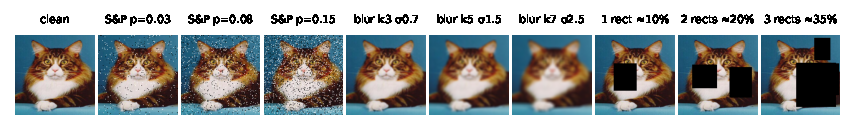
\includegraphics[width=0.8\textwidth]{corruption_grid.pdf}
\caption{The ten deterministic test conditions for one test image (clean and three severities of each corruption).}\label{fig:corr}
\end{figure*}

\textbf{Manifests.} Validation (736 entries, 184 per class) and test manifests are generated once and store the corruption type, severity, parameters, mask coordinates and seed, with a SHA-256 digest. Every test image appears under all ten conditions, giving \textbf{36,690 test inputs} (3,669 images $\times$ 10); all test tables use this full manifest.

\textbf{FS2K (Task 4).} The official training/test definitions are used. 15\% of the training portion is held out as validation, stratified by style with seed 42, leaving \textbf{899 training and 159 validation pairs}; the \textbf{1,046 official test pairs} (619, 381 and 46 in styles 1, 2, 3) are used only for the final evaluation. Photographs are $128\times128$ RGB, sketches $128\times128$ grayscale; augmentation (flip, random crop-and-resize) is applied identically to both members of a pair.

\textbf{Metrics.} L1 (images in $[0,1]$), SSIM (11-pixel Gaussian window) and PSNR in dB, clipped at 60\,dB because identical images give infinite PSNR. The score of the untouched corrupted input (``no restoration'') is always shown, since a restoration model is useful only where it beats it. Classification uses accuracy, macro precision/recall/F1, per-class values and a row-normalised confusion matrix.

\section{Task 1: Universal Multi-Corruption Denoising Autoencoder}\label{sec:t1}

\subsection{Architecture}
The network (Fig.~\ref{fig:arch1}) has a convolutional encoder, a compressed latent, and a convolutional decoder, and receives no information about the corruption type. The encoder halves the spatial size four times ($128\to8$) while widening the channels ($48,96,192,384$); each stage is a stride-2 $3\times3$ convolution followed by a $3\times3$ convolution, both with batch normalisation and ReLU. A $1\times1$ convolution projects to a \emph{linear} latent $z$ of $32\times8\times8=2{,}048$ values (4.2\% of the $49{,}152$ pixel values), followed by Dropout2d. The decoder mirrors the encoder with nearest-neighbour $2\times$ upsampling and $3\times3$ convolutions and ends in a $3\times3$ convolution with a sigmoid. There are \textbf{no skip connections}: every pixel of the output must be generated from $z$. The model has 4.01\,M parameters.

\begin{figure*}[t]
\centering
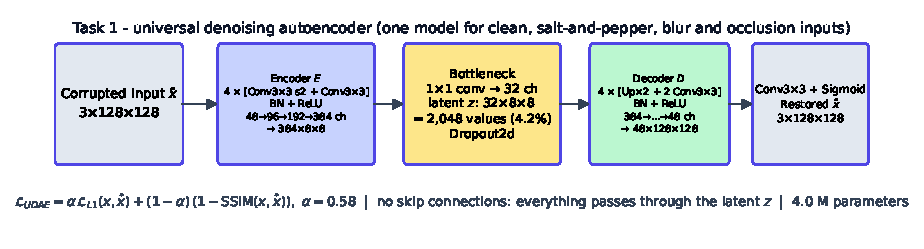
\includegraphics[width=\textwidth]{arch_task1.pdf}
\caption{Universal denoising autoencoder. The only path from input to output goes through the 2,048-value latent.}\label{fig:arch1}
\end{figure*}

\subsection{Loss and training}
With $\hat{x}=D(E(\tilde{x}))$ the loss is
\begin{equation}
\mathcal{L}_{UDAE}=\alpha\,\mathcal{L}_{1}(x,\hat{x})+(1-\alpha)\bigl(1-\mathrm{SSIM}(x,\hat{x})\bigr),
\end{equation}
where L1 encourages accurate pixels and SSIM preserves structure and local contrast. Optuna selected $\alpha=0.58$ (the suggested starting value was 0.8). Training uses AdamW (weight decay $10^{-4}$), a cosine learning-rate schedule, gradient clipping at 1.0, mixed precision on an NVIDIA T4, batch 16 and learning rate $4.6\times10^{-4}$ for 100 epochs over all 2,944 training images, each drawn with a fresh random corruption. The checkpoint with the lowest validation objective $0.5\,\mathcal{L}_1+0.5\,(1-\mathrm{SSIM})$ is kept (epoch \nTOneBestEpoch{}); this objective does not depend on $\alpha$ and is therefore comparable across trials. The search space, trial counts and selected values are in Section~\ref{sec:optuna}.

\subsection{A first attempt that under-fitted}
Our first complete run (search space with dropout up to 0.3, latent sizes 16--128, three-epoch trials on 600 images, then 30 epochs on 736 images) was measured on the single-condition test manifest and reached only SSIM \nAttemptOneSSIM{} and PSNR \nAttemptOnePSNR{}\,dB. Two observations identified the cause. First, the train--validation gap was only 0.008 SSIM: the model was not memorising, it was \emph{under-fitting}. Second, clean, blurred and noisy inputs all scored about 0.55--0.56 SSIM, so even clean images were reconstructed no better than corrupted ones: the limit was the model's ability to reconstruct at all. Optuna had chosen dropout $0.29$ (dropout in an autoencoder deletes the very features needed for reconstruction) and the largest allowed latent, because three-epoch trials reward configurations that learn fast early. We therefore capped the dropout at 0.15, added latent sizes up to 256, lengthened trials to six epochs, and trained the final model for 100 epochs on all training data. On the same manifest the SSIM rose from \nAttemptOneSSIM{} to \nTOneSSIMsingle{}.

\subsection{Results}
Table~\ref{tab:task1} gives the results on the full test protocol, separated by corruption and by severity, next to the score of the untouched corrupted input (``no restoration''), which any useful restoration must beat. Figure~\ref{fig:bars} summarises all three restoration systems.

\begin{table*}[t]
\centering
\caption{Task 1 (universal autoencoder) on the \nNEntries{} deterministic test inputs. PSNR is clipped at 60\,dB ($\geq$60 for the identical clean input).}\label{tab:task1}
\small
\adjustbox{max width=\textwidth}{\begin{tabular}{llcccccr}
\toprule
 & & & \multicolumn{2}{c}{Input (no restoration)} & \multicolumn{3}{c}{Universal autoencoder} \\
\cmidrule(lr){4-5}\cmidrule(lr){6-8}
Corruption & Setting & Level & SSIM & PSNR & L1 & SSIM & PSNR \\
\midrule
clean & -- & -- & 1.000 & $\geq$60 & 0.036 & 0.814$\pm$0.080 & 25.97 \\
salt-and-pepper & $p{=}0.03$ & low & 0.602 & 20.13 & 0.036 & 0.813$\pm$0.080 & 25.95 \\
salt-and-pepper & $p{=}0.08$ & medium & 0.339 & 15.87 & 0.036 & 0.808$\pm$0.081 & 25.89 \\
salt-and-pepper & $p{=}0.15$ & high & 0.204 & 13.14 & 0.037 & 0.796$\pm$0.082 & 25.68 \\
Gaussian blur & $k{=}3,\sigma{=}0.7$ & low & 0.944 & 32.34 & 0.035 & 0.814$\pm$0.081 & 26.17 \\
Gaussian blur & $k{=}5,\sigma{=}1.5$ & medium & 0.806 & 26.77 & 0.036 & 0.805$\pm$0.083 & 26.04 \\
Gaussian blur & $k{=}7,\sigma{=}2.5$ & high & 0.692 & 24.35 & 0.039 & 0.751$\pm$0.097 & 25.13 \\
occlusion & 1 rect, 10\% & low & 0.861 & 16.67 & 0.043 & 0.768$\pm$0.083 & 23.56 \\
occlusion & 2 rects, 20\% & medium & 0.730 & 13.34 & 0.051 & 0.718$\pm$0.086 & 21.66 \\
occlusion & 3 rects, 35\% & high & 0.547 & 10.77 & 0.067 & 0.634$\pm$0.091 & 19.21 \\
\midrule
\multicolumn{3}{l}{all corrupted (33,021)} & 0.636 & 19.27 & 0.042 & 0.767 & 24.36 \\
\multicolumn{3}{l}{all conditions (36,690)} & 0.672 & 23.34 & 0.042 & 0.772 & 24.52 \\
\bottomrule
\end{tabular}
}
\end{table*}

\begin{figure}[t]
\centering
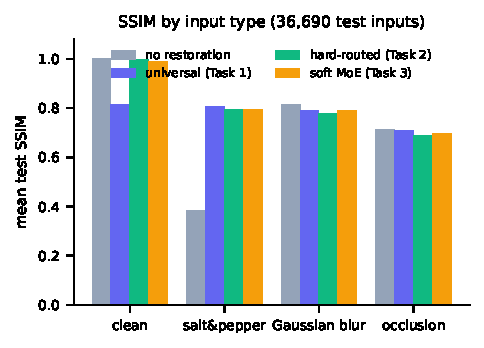
\includegraphics[width=\columnwidth]{bar_comparison.pdf}
\caption{Mean test SSIM per input type for the corrupted input, the universal autoencoder, hard routing and the soft mixture.}\label{fig:bars}
\end{figure}

\textbf{Salt-and-pepper noise is restored well.} SSIM rises from \nInputSSIMsaltpepper{} to \nTOneSSIMsaltpepper{} and PSNR from \nInPSNRsaltpepper{} to \nTOnePSNRsaltpepper{}\,dB; the output quality is almost independent of severity (0.813 to 0.796 SSIM from $p=0.03$ to $p=0.15$), because the noise is removed by averaging over the many uncorrupted neighbours.

\textbf{Blur is not helped, and clean images are damaged.} For Gaussian blur the output scores \nTOneSSIMblur{} SSIM and \nTOnePSNRblur{}\,dB while the untouched input already scores \nInputSSIMblur{} and \nInPSNRblur{}\,dB; at $k=5$ the two tie (0.805 against 0.806) and only for the strongest blur ($k=7$) does restoration beat the input in SSIM (0.751 against 0.692). Clean images fall from 1.000 to \nTOneSSIMclean{}. The bottleneck cannot reproduce fine detail, so mild blur is ``restored'' into a slightly different soft image. This is the central limitation of the universal design and the motivation for Tasks~2 and~3: an identity path costs nothing on inputs that do not need restoration.

\textbf{Occlusion: SSIM and PSNR disagree.} Overall the output scores \nTOneSSIMocclusion{} SSIM against \nInputSSIMocclusion{} for the masked input, yet PSNR rises from \nInPSNRocclusion{} to \nTOnePSNRocclusion{}\,dB. SSIM is computed in local windows, so the large part of the image outside the black rectangles is already perfect and the mean SSIM of the untouched input stays high; doing nothing scores a higher SSIM than the autoencoder on \nOccNoneBetterLow\% of the low-severity (10\%), \nOccNoneBetterMedium\% of the medium and \nOccNoneBetterHigh\% of the high-severity inputs. PSNR and visual inspection (Fig.~\ref{fig:ex1}) show what SSIM hides: the autoencoder replaces the black holes by plausible content, which removes the large pixel errors inside the mask. Only at 35\% coverage does restoration also win in SSIM (0.634 against 0.547). We therefore read both measures together.

\textbf{Generalisation.} On 736 training images corrupted with validation-style fixed corruptions the SSIM is \nTrainSSIMsub{}, against \nValSSIMsub{} on the 736 unseen validation images (gap \nGapSSIM{}); training and validation curves (Fig.~\ref{fig:curves1}) move together, so the model neither memorises nor over-fits.

\begin{figure*}[t]
\centering
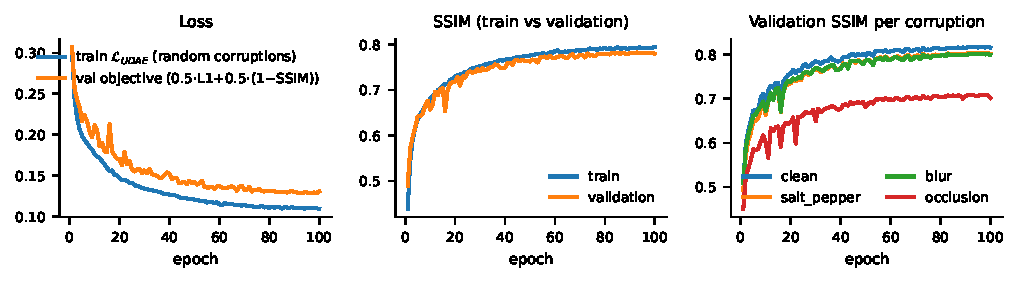
\includegraphics[width=\textwidth]{curves_task1.pdf}
\caption{Task 1 training and validation curves (100 epochs). Validation SSIM is reported separately for each corruption.}\label{fig:curves1}
\end{figure*}

\begin{figure*}[t]
\centering
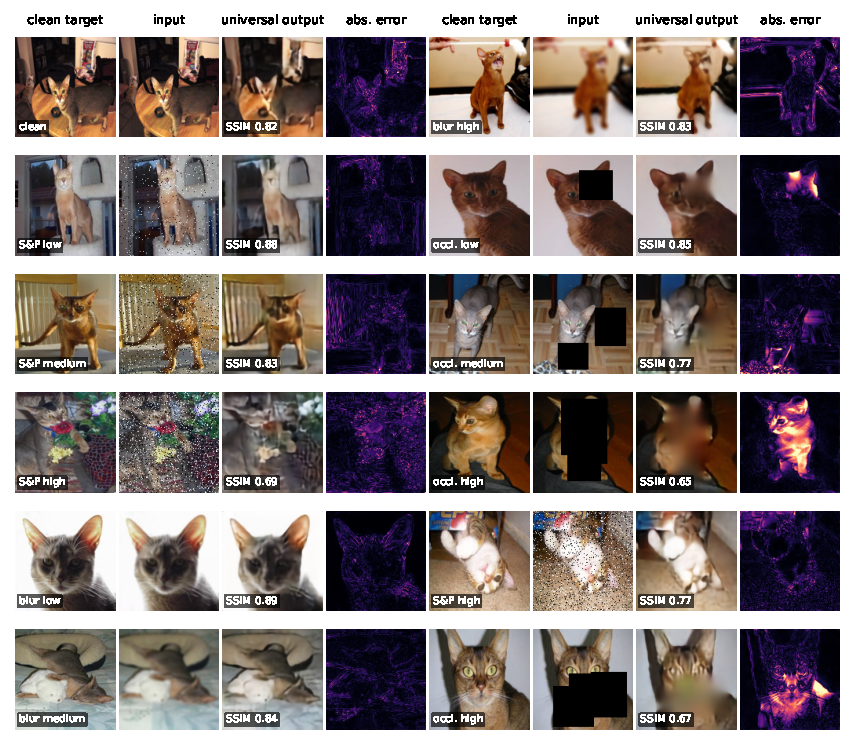
\includegraphics[width=0.94\textwidth]{examples_universal.pdf}
\caption{Twelve representative test inputs for the universal autoencoder: clean target, corrupted input, output with its SSIM, and the absolute error map (every condition appears at least once).}\label{fig:ex1}
\end{figure*}

\begin{figure}[t]
\centering
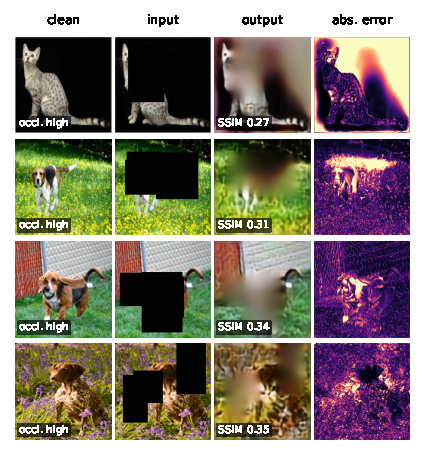
\includegraphics[width=\columnwidth]{failure_universal.pdf}
\caption{The four lowest-SSIM corrupted test inputs for the universal autoencoder.}\label{fig:fail1}
\end{figure}

\textbf{Failure cases.} Figure~\ref{fig:fail1} shows the four worst corrupted inputs; all are 35\% occlusions. In the first, a cat on a black background, the mask merges with the background and cuts the animal in two; the network reconstructs a smeared grey-brown shape (SSIM 0.27). In the second, the three rectangles cover the head and back of a dog on grass; the output is a blurred brown-green patch without the animal (0.31). In the third, an L-shaped mask removes the head of a basset hound and the network paints wall and grass texture instead (0.34). In the fourth, two masks cover the body of a brown dog and a third one the top right (0.35). In all four the error is concentrated inside the masks and along the animal's outline: the information is absent, so the best the autoencoder can do is a smooth guess that matches the surroundings; it cannot reconstruct the subject.

\section{Task 2: Classification and Hard-Routed Specialists}\label{sec:t2}

\begin{figure*}[t]
\centering
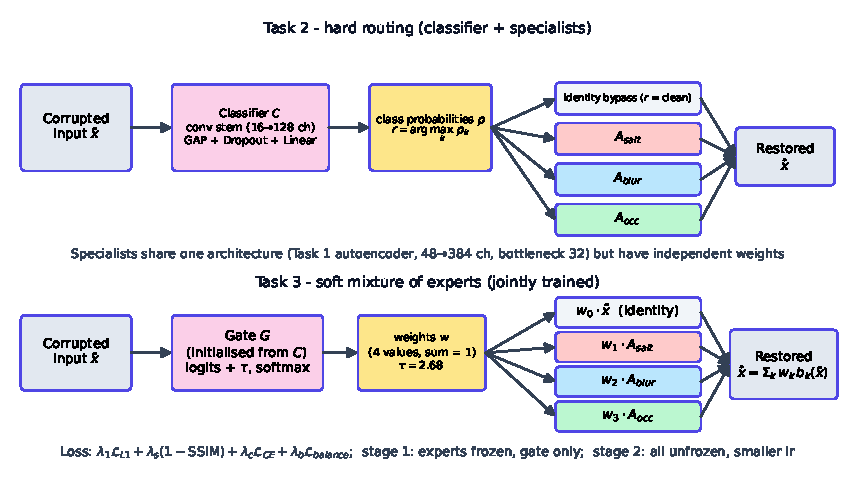
\includegraphics[width=0.6\textwidth]{arch_task2_task3.pdf}
\caption{Top: hard routing (Task~2); the classifier output $r$ selects a specialist or the identity bypass. Bottom: the soft mixture of experts (Task~3) built from the same components.}\label{fig:arch23}
\end{figure*}

\textbf{Classifier.} Four stride-2 stages of two $3\times3$ convolutions (16--128 channels, batch norm, ReLU, Dropout2d), global average pooling, dropout and a linear layer give $p=[p_{clean},p_{salt},p_{blur},p_{occ}]$ with 0.295\,M parameters and $r=\arg\max_k p_k$. It is trained with multiclass cross-entropy on exactly balanced batches; Optuna tuned learning rate, batch size, channel configuration, dropout and weight decay (objective: validation macro-F1), selecting learning rate $1.5\times10^{-3}$, batch 32, dropout 0.15, weight decay $1.3\times10^{-4}$, 30 epochs. On the test protocol it reaches accuracy \nClfAcc{} and macro-F1 \nClfMacroF{} (Table~\ref{tab:classifier}, Fig.~\ref{fig:cm}). Salt-and-pepper is recognised perfectly; the \nMisrouteCount{} errors (\nMisroute\%) are clean images taken for blurred or occluded ones, and low-severity occlusions taken for clean images.

\begin{table}[t]
\centering
\caption{Classifier metrics on the test protocol.}\label{tab:classifier}
\small
\adjustbox{max width=\columnwidth}{\begin{tabular}{lrccc}
\toprule
Class & Support & Precision & Recall & F1 \\
\midrule
clean & 3,669 & 0.965 & 0.977 & 0.971 \\
salt-and-pepper & 11,007 & 1.000 & 1.000 & 1.000 \\
Gaussian blur & 11,007 & 0.994 & 1.000 & 0.997 \\
occlusion & 11,007 & 0.998 & 0.988 & 0.993 \\
\midrule
macro average & 36,690 & 0.989 & 0.991 & 0.990 \\
\multicolumn{2}{l}{overall accuracy} & \multicolumn{3}{c}{0.9941} \\
\bottomrule
\end{tabular}
}
\end{table}

\begin{figure}[t]
\centering
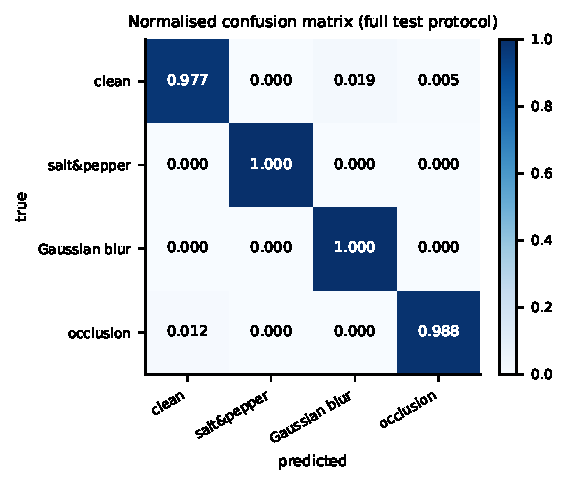
\includegraphics[width=0.75\columnwidth]{confusion_matrix.pdf}
\caption{Row-normalised confusion matrix of the classifier.}\label{fig:cm}
\end{figure}

\textbf{Specialists.} Three autoencoders $A_{salt}$, $A_{blur}$, $A_{occ}$ share the Task~1 architecture but have independent parameters, each trained only on its own corruption with the same clean target. As the assignment allows, one shared Optuna search (each trial trains all three for six epochs on 1,000 images) selects a common configuration (learning rate $6.8\times10^{-4}$, batch 32, dropout 0.07, $\alpha=0.60$); the specialists are then trained for 100 epochs. Inference is
\begin{equation}
\hat{x}=\begin{cases}\tilde{x}, & r=\text{clean},\\ A_{salt}(\tilde{x}), & r=\text{salt},\\ A_{blur}(\tilde{x}), & r=\text{blur},\\ A_{occ}(\tilde{x}), & r=\text{occlusion},\end{cases}
\end{equation}
so clean inputs take an identity bypass. \emph{Oracle} routing (true label) measures the specialists; \emph{predicted} routing measures the deployable system.

\textbf{Colour loss and its correction.} The first specialists (Optuna chose $\alpha=0.29$) produced washed-out, sepia-toned images, which we noticed when inspecting the outputs. Colourfulness measured on \nColourN{} salt-and-pepper test inputs confirmed it (Table~\ref{tab:colour}): the first specialist kept \nColSpSpecFirst\% of the colour and the first mixture \nColSpMoeFirst\%, the universal model \nColSpUniversal\%. SSIM is weakly sensitive to a global chroma shift, so neither the loss nor the Optuna objective penalised it. We restricted $\alpha$ to $[0.55,0.95]$ and retrained the specialists and the mixture: the final specialist keeps \nColSpSpecFinal\% and the mixture \nColSpMoeFinal\%; the L1 error of the routed system fell by \nLOneDropPct\% (\nHardPredLOneFirst{} to \nHardPredLOneFinal{}) with SSIM essentially unchanged. The occlusion specialist still keeps slightly less colour than the universal model (\nColOcSpecFinal\% against \nColOcUniversal\%).

\begin{table}[t]
\centering
\caption{Colour preserved (colourfulness of the output relative to the clean image) on \nColourN{} salt-and-pepper and occlusion test inputs.}\label{tab:colour}
\small
\adjustbox{max width=\columnwidth}{\begin{tabular}{lcc}
\toprule
Model output & salt-and-pepper inputs & occlusion inputs \\
\midrule
clean image (reference) & 100\% & 100\% \\
corrupted input & 91\% & 77\% \\
universal AE (Task 1) & 97\% & 96\% \\
specialist, first run ($\alpha\approx0.3$) & 43\% & 79\% \\
specialist, final ($\alpha\approx0.6$) & 89\% & 88\% \\
soft MoE, first run ($\alpha\approx0.3$) & 46\% & 94\% \\
soft MoE, final ($\alpha\approx0.6$) & 97\% & 94\% \\
\bottomrule
\end{tabular}
}
\end{table}

\begin{table*}[t]
\centering
\caption{Hard routing on the test protocol: SSIM and L1 of oracle versus predicted routing, and the share of mis-routed inputs.}\label{tab:routing}
\small
\adjustbox{max width=\textwidth}{\begin{tabular}{lccccccc}
\toprule
 & \multicolumn{3}{c}{SSIM} & & \multicolumn{2}{c}{L1} & \\
\cmidrule(lr){2-5}\cmidrule(lr){6-7}
Input type & no restoration & universal & oracle & predicted & oracle & predicted & misroute \% \\
\midrule
clean & 1.000 & 0.814 & 1.000 & 0.996 & 0.0000 & 0.0010 & 2.34 \\
salt-and-pepper & 0.382 & 0.805 & 0.793 & 0.793 & 0.0444 & 0.0444 & 0.00 \\
Gaussian blur & 0.814 & 0.790 & 0.780 & 0.780 & 0.0449 & 0.0449 & 0.01 \\
occlusion & 0.713 & 0.707 & 0.689 & 0.690 & 0.0597 & 0.0594 & 1.19 \\
\midrule
all (36,690) & 0.672 & 0.772 & 0.779 & 0.779 & 0.0447 & 0.0447 & 0.59 \\
\bottomrule
\end{tabular}
}
\end{table*}

\textbf{Routing results.} Predicted routing (SSIM \nHardPredSSIM{}) is indistinguishable from oracle routing (\nHardOracleSSIM{}) because the classifier is accurate (Table~\ref{tab:routing}). Its advantage over the universal model (\nTOneSSIMall{}) comes entirely from clean images (\nHardSSIMclean{} against \nTOneSSIMclean{}). On corrupted inputs the specialists are slightly \emph{worse} than the universal model: \nHardSSIMsaltpepper{} against \nTOneSSIMsaltpepper{} for noise, \nHardSSIMblur{} against \nTOneSSIMblur{} for blur and \nHardSSIMocclusion{} against \nTOneSSIMocclusion{} for occlusion. A specialist has the same capacity and bottleneck as the universal model, so specialisation adds no reconstruction ability, and one shared search for three models and a batch of 32 (half the updates per epoch) may explain the small gap. The measured benefit of routing is the identity bypass.

\begin{figure*}[t]
\centering
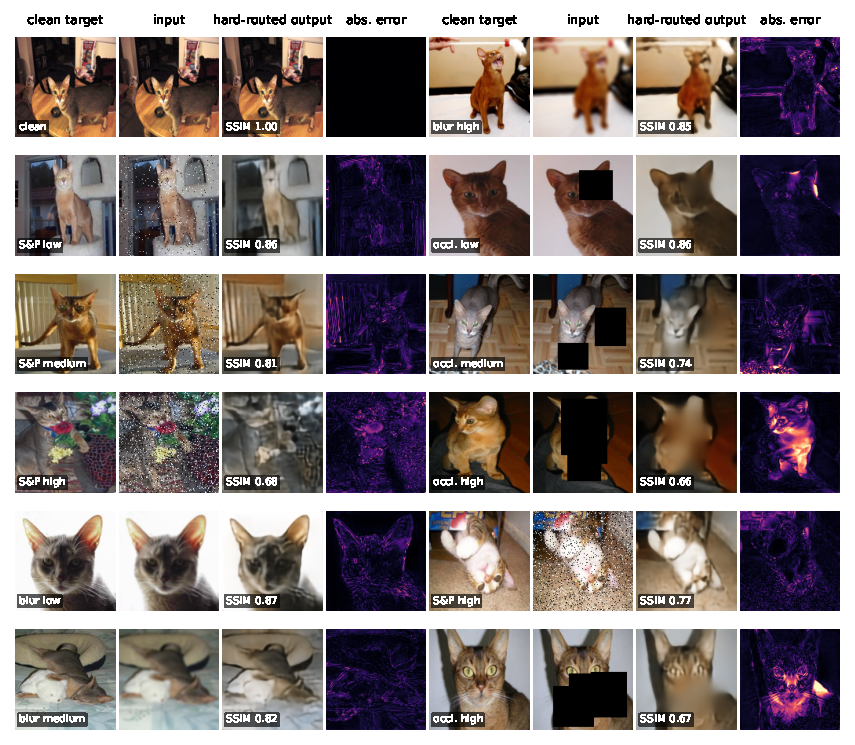
\includegraphics[width=0.52\textwidth]{examples_hard.pdf}
\caption{Twelve test inputs for hard-routed restoration (predicted routing).}\label{fig:ex2}
\end{figure*}

\begin{figure}[t]
\centering
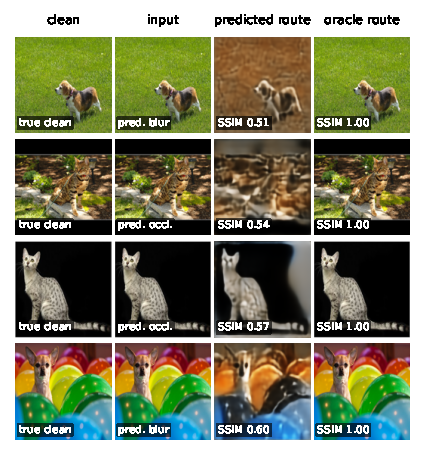
\includegraphics[width=0.85\columnwidth]{misroute_hard.pdf}
\caption{Classifier-induced failures: the four mis-routed clean images with the largest SSIM loss; predicted route next to oracle route.}\label{fig:mis}
\end{figure}

\begin{figure*}[t]
\centering
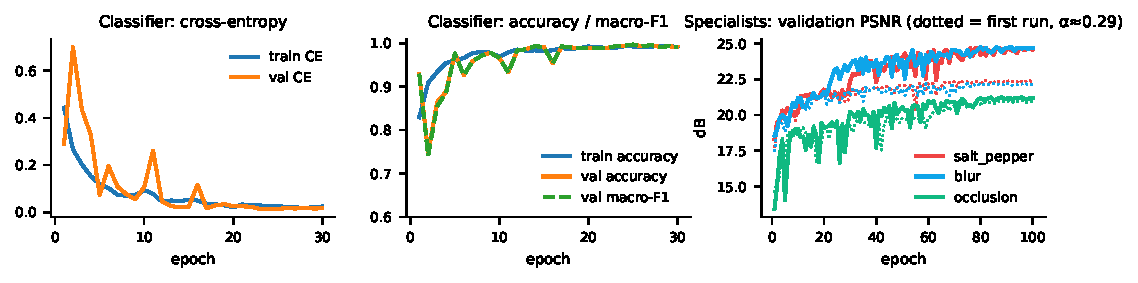
\includegraphics[width=0.7\textwidth]{curves_task2.pdf}
\caption{Task 2 training curves: classifier loss and accuracy, and validation PSNR of the three specialists in the first (dotted) and final (solid) run.}\label{fig:curves2}
\end{figure*}

\textbf{Classifier-caused failures.} The \nMisClean{} clean images sent to a blur or occlusion expert are real failures (SSIM \nMisCleanLoss{} on average relative to the oracle route). In Fig.~\ref{fig:mis} a clean dog on grass is taken for blurred and ``restored'' into a smeared brown scene (0.51 instead of 1.00), and an image with black letterbox bars and a cat on a black background are taken for occluded, so the occlusion expert invents content for the dark regions (0.54, 0.57). Conversely, 128 occlusions labelled ``clean'' (126 of them 10\% masks) are left untouched; this scores about $+0.12$ SSIM \emph{higher}, but only because SSIM ignores the black rectangle, which stays visible. Overall, mis-routing changes mean SSIM by only $+0.0001$ because the two groups cancel. The four worst outputs of the system are, as for Task~1, 35\% occlusions that hide the animal (SSIM 0.28--0.33); they are not routing errors, and the occlusion specialist fills the hole with a brownish patch even where the surroundings are green.

\section{Task 3: Jointly Trained Soft Mixture of Experts}\label{sec:t3}

\subsection{Model and losses}
Hard routing fails when the classifier is uncertain or when two corruptions mix. The soft model (Fig.~\ref{fig:arch23}, bottom) replaces the decision by a differentiable combination. A gate $G$ with the classifier's architecture produces weights
\begin{equation}
w=\mathrm{softmax}\bigl(G(\tilde{x})/\tau\bigr),\qquad \hat{x}=w_0\tilde{x}+w_1A_{salt}(\tilde{x})+w_2A_{blur}(\tilde{x})+w_3A_{occ}(\tilde{x}),
\end{equation}
where branch~0 is the identity and $\tau$ controls whether the weights are sharp or spread out. Because the mixture is differentiable, gate and experts are trained jointly from the reconstruction error. The components are \emph{not} initialised randomly: the gate starts from the trained Task~2 classifier and the experts from the final specialists. Training has two stages: a short warm-up (2 epochs, learning rate $10^{-3}$) in which the experts are frozen, in evaluation mode, and only the gate is trained, followed by 30 epochs of joint fine-tuning with a much smaller learning rate. The loss is
\begin{equation}
\mathcal{L}_{MoE}=\lambda_1\mathcal{L}_{1}+\lambda_s(1-\mathrm{SSIM})+\lambda_c\mathcal{L}_{CE}+\lambda_b\mathcal{L}_{balance},
\end{equation}
with $\mathcal{L}_{balance}=\sum_{k=0}^{3}(\bar{w}_k-\tfrac14)^2$, where $\bar{w}_k$ is the mean weight of branch $k$ in a mini-batch. The cross-entropy acts on the raw gate logits, which keeps the question ``does the gate know the true class'' separate from ``how sharply does it mix'' (the temperature). We tie $\lambda_1=\alpha$ and $\lambda_s=1-\alpha$, so that the five quantities Optuna tuned (joint learning rate, temperature, $\lambda_c$, $\lambda_b$ and the L1/SSIM weighting $\alpha$) map one-to-one onto the assignment's list and the reconstruction weights cannot both shrink to zero. The selected values are $\tau=2.68$, $\lambda_c=0.48$, $\lambda_b=1.20$, $\alpha=0.61$ and a joint learning rate of $4.3\times10^{-5}$; median pruning removed half of the trials (Section~\ref{sec:optuna}). The first mixture (with $\alpha=0.32$) inherited the colour loss of its experts, and the final one was retrained from the corrected specialists (Section~\ref{sec:colour}).

\begin{figure*}[t]
\centering
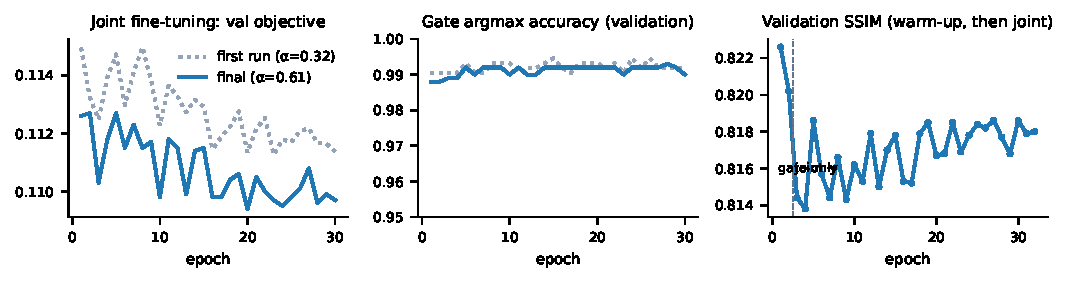
\includegraphics[width=\textwidth]{curves_task3.pdf}
\caption{Task 3 training: validation objective and gate accuracy for the first (dotted) and final runs, and validation SSIM over the warm-up and joint stages of the final run.}\label{fig:curves3}
\end{figure*}

\subsection{Reconstruction results}
Table~\ref{tab:task3} compares the three restoration systems on every test condition. The soft mixture reaches an overall SSIM of \nSoftSSIM{} against \nHardPredSSIM{} for predicted hard routing and \nTOneSSIMall{} for the universal model. Clean images stay almost untouched (SSIM \nSoftSSIMclean{}) because the gate puts most of its weight on the identity branch. On the corrupted types the mixture is on par with hard routing and with the universal model (overall \nSoftSSIMsaltpepper{} for noise, \nSoftSSIMblur{} for blur and \nSoftSSIMocclusion{} for occlusion, PSNR \nSoftPSNRsaltpepper{}, \nSoftPSNRblur{} and \nSoftPSNRocclusion{}\,dB); it is slightly better than hard routing at the low severities (for example blur $k=3$: 0.820 against 0.792) and slightly worse at the high ones (noise $p=0.15$: 0.778 against 0.790), which is what a smoother, less committed decision would be expected to do. Blending experts does not remove the fundamental limit on heavy occlusion.

\begin{table*}[t]
\centering
\caption{Soft mixture of experts (Task~3) compared with the universal model and predicted hard routing on the full test protocol.}\label{tab:task3}
\small
\adjustbox{max width=\textwidth}{\begin{tabular}{llcccrr}
\toprule
 & & \multicolumn{3}{c}{SSIM} & \multicolumn{2}{c}{soft MoE} \\
\cmidrule(lr){3-5}\cmidrule(lr){6-7}
Corruption & Level & universal & hard (pred.) & soft MoE & L1 & PSNR (dB) \\
\midrule
clean & -- & 0.814 & 0.996 & 0.991$\pm$0.017 & 0.0081 & 40.19 \\
salt-and-pepper & low & 0.813 & 0.796 & 0.807$\pm$0.070 & 0.0427 & 24.98 \\
salt-and-pepper & medium & 0.808 & 0.794 & 0.795$\pm$0.075 & 0.0436 & 24.83 \\
salt-and-pepper & high & 0.796 & 0.790 & 0.778$\pm$0.075 & 0.0441 & 24.71 \\
Gaussian blur & low & 0.814 & 0.792 & 0.820$\pm$0.074 & 0.0400 & 25.55 \\
Gaussian blur & medium & 0.805 & 0.790 & 0.795$\pm$0.086 & 0.0424 & 25.04 \\
Gaussian blur & high & 0.751 & 0.757 & 0.754$\pm$0.096 & 0.0448 & 24.49 \\
occlusion & low & 0.768 & 0.747 & 0.771$\pm$0.083 & 0.0484 & 22.78 \\
occlusion & medium & 0.718 & 0.699 & 0.699$\pm$0.093 & 0.0575 & 21.28 \\
occlusion & high & 0.634 & 0.625 & 0.621$\pm$0.098 & 0.0718 & 19.16 \\
\midrule
all (36,690) & & 0.772 & 0.779 & 0.783$\pm$0.120 & 0.0443 & 25.30 \\
\bottomrule
\end{tabular}
}
\end{table*}

\subsection{Behaviour of the gating network}
\textbf{Average weights.} Table~\ref{tab:gate} and Fig.~\ref{fig:heat} give the mean routing weight of each branch for every true corruption and severity. The gate is well aligned with the truth: the matching expert receives on average \nHomeWeightSalt{} of the weight for salt-and-pepper, \nHomeWeightBlur{} for blur and \nHomeWeightOcc{} for occlusion, and the identity branch \nHomeWeightClean{} for clean images. The weight grows with severity (occlusion: from \nGateOccLow{} at 10\% coverage to \nGateOccHigh{} at 35\%), as it should, since heavier corruption is easier to recognise. Weights are not one-hot because the temperature (2.68) deliberately spreads them: the mean largest weight is \nGateMaxMean{}.

\begin{table}[t]
\centering
\caption{Mean gate weights by true condition (full test protocol).}\label{tab:gate}
\small
\adjustbox{max width=\columnwidth}{\begin{tabular}{lcccc l}
\toprule
True condition & $w_0$ identity & $w_1$ salt & $w_2$ blur & $w_3$ occl. & dominant \\
\midrule
clean  & 0.808 & 0.030 & 0.098 & 0.063 & clean \\
salt-and-pepper low & 0.052 & 0.838 & 0.076 & 0.034 & salt-and-pepper \\
salt-and-pepper medium & 0.041 & 0.865 & 0.068 & 0.026 & salt-and-pepper \\
salt-and-pepper high & 0.042 & 0.864 & 0.067 & 0.027 & salt-and-pepper \\
Gaussian blur low & 0.148 & 0.017 & 0.807 & 0.028 & Gaussian blur \\
Gaussian blur medium & 0.096 & 0.014 & 0.865 & 0.025 & Gaussian blur \\
Gaussian blur high & 0.096 & 0.014 & 0.864 & 0.025 & Gaussian blur \\
occlusion low & 0.108 & 0.064 & 0.028 & 0.800 & occlusion \\
occlusion medium & 0.012 & 0.026 & 0.005 & 0.958 & occlusion \\
occlusion high & 0.002 & 0.009 & 0.001 & 0.988 & occlusion \\
\bottomrule
\end{tabular}
}
\end{table}

\begin{figure}[t]
\centering
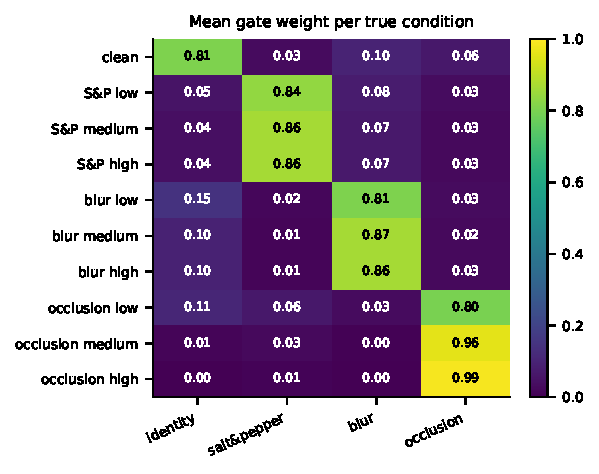
\includegraphics[width=\columnwidth]{gate_heatmap.pdf}
\caption{Routing heat-map: mean weight of each branch for each true corruption and severity.}\label{fig:heat}
\end{figure}

\textbf{Dominant versus distributed routing.} Figure~\ref{fig:soft} contrasts inputs on which one expert dominates (left: the most ``one-expert'' input of each corruption) with inputs on which the weights are spread (right). The spread-out cases are low-severity corruptions, for which the image is close to a clean one and the identity and expert branches are both plausible: the mean weight entropy is \nEntOccLow{} nats for 10\% occlusions and \nEntClean{} for clean images, against only \nEntOccHigh{} for 35\% occlusions, where the gate is nearly one-hot (Table~\ref{tab:gate}). For such inputs the mixture yields a smoother output than a hard decision would.

\begin{figure*}[t]
\centering
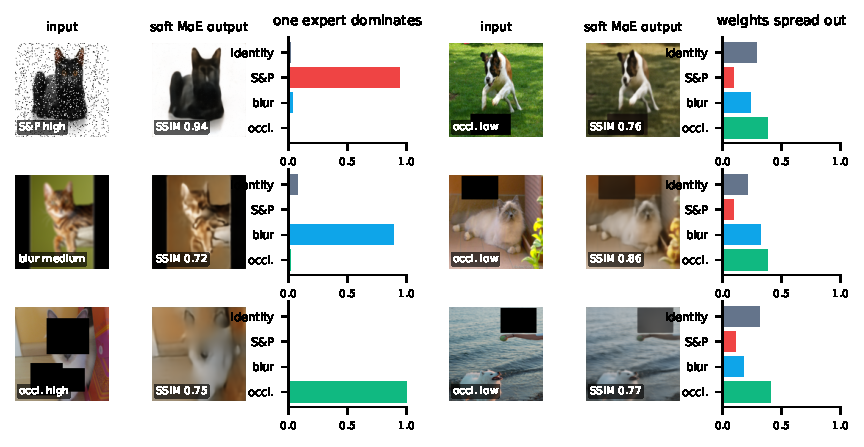
\includegraphics[width=0.94\textwidth]{soft_weights_examples.pdf}
\caption{Left: inputs for which a single expert dominates the mixture. Right: inputs for which the weights are distributed over several branches.}\label{fig:soft}
\end{figure*}

\textbf{Inactive or dominant experts.} Table~\ref{tab:dominance} lists, for each true type, the percentage of inputs on which each branch has the largest weight. No branch is dead: each branch is the top branch for a substantial share of inputs (overall: identity \nTopShareclean{}\%, salt-and-pepper \nTopSharesaltpepper{}\%, blur \nTopShareblur{}\%, occlusion \nTopShareocclusion{}\%), and no branch dominates unrelated inputs, so the balance regulariser did its job without forcing a uniform mixture.

\begin{table}[t]
\centering
\caption{Dominance analysis: where each branch has the largest weight.}\label{tab:dominance}
\small
\adjustbox{max width=\columnwidth}{\begin{tabular}{lccccc}
\toprule
True type & \multicolumn{4}{c}{\% of inputs where branch has the largest weight} & mean max weight \\
\cmidrule(lr){2-5}
 & identity & salt & blur & occl. & \\
\midrule
clean & 99.1 & 0.0 & 0.7 & 0.2 & 0.811 \\
salt-and-pepper & 0.0 & 100.0 & 0.0 & 0.0 & 0.856 \\
Gaussian blur & 0.0 & 0.0 & 100.0 & 0.0 & 0.846 \\
occlusion & 1.9 & 0.0 & 0.0 & 98.0 & 0.921 \\
\midrule
all inputs & 10.5 & 30.0 & 30.1 & 29.4 & 0.868 \\
\bottomrule
\end{tabular}
}
\end{table}

\begin{figure*}[t]
\centering
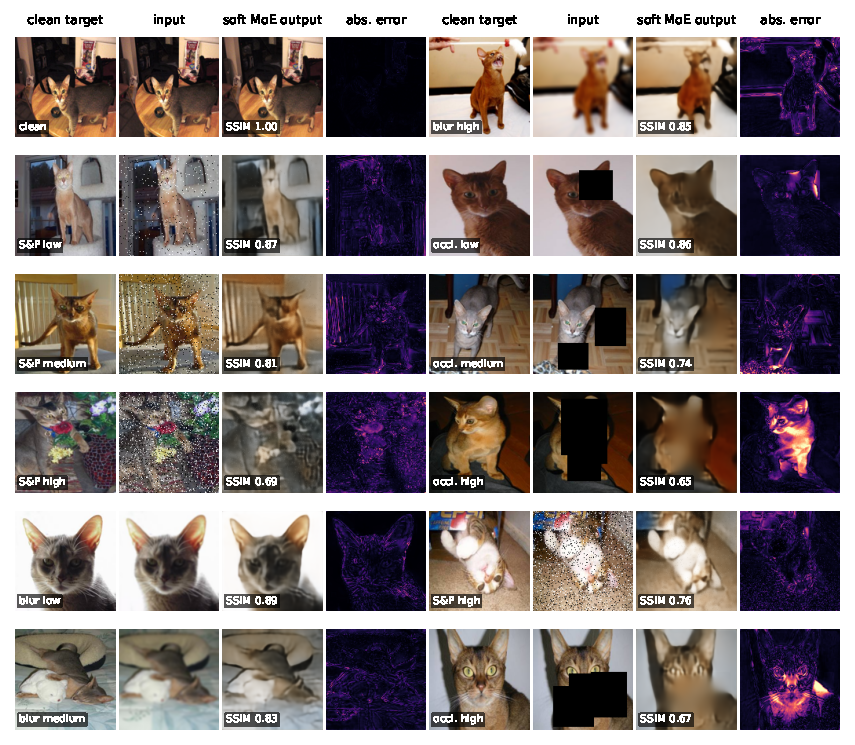
\includegraphics[width=0.94\textwidth]{examples_soft.pdf}
\caption{Twelve representative test inputs for the soft mixture of experts.}\label{fig:ex3}
\end{figure*}

\begin{figure}[t]
\centering
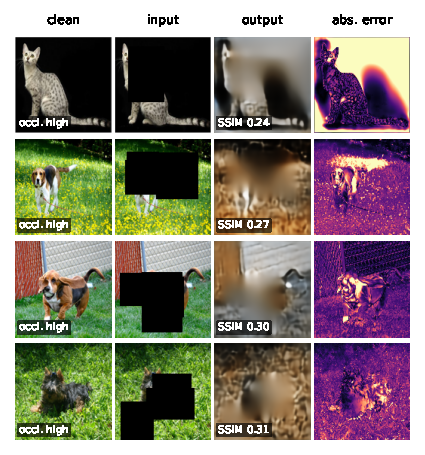
\includegraphics[width=\columnwidth]{failure_soft.pdf}
\caption{The four lowest-SSIM corrupted test inputs for the soft mixture.}\label{fig:fail3}
\end{figure}

\textbf{Failure cases.} Figure~\ref{fig:fail3} shows the four worst outputs of the mixture (SSIM 0.24--0.31). They are the same kind of input as for the other systems: 35\% occlusions that hide the subject. The first is the cat on a black background whose black mask merges with the background, so the input looks like a half-empty image and the mixture produces a grey-brown cloud; in the other three (a beagle, a basset hound and a dark terrier on grass) the gate gives the occlusion expert nearly all of the weight, which is the correct routing, but the expert cannot recreate the animal. The worst cases of the mixture are about 0.03--0.04 SSIM below those of the universal model (0.24--0.31 against 0.27--0.35). Because the information is absent, no routing or blending strategy can recover these inputs, and all three systems produce a smooth, plausible fill instead of the subject.

\section{Task 4: Style-Conditioned Face-to-Sketch cGAN}\label{sec:t4}

\subsection{Model}
The generator $\hat{y}=G(x,s)$ (Fig.~\ref{fig:arch4}) is a U-Net~\cite{ronneberger2015}: seven stride-2 encoder blocks (64, 128, 256, 512 channels, four times 512 at the deepest levels) reduce the $128\times128$ photograph to a $1\times1$ code, and six transposed-convolution blocks with skip connections restore the resolution; a final transposed convolution with tanh produces a one-channel sketch. The first three decoder blocks use dropout (0.30). The style $s\in\{1,2,3\}$ is a \emph{learned categorical embedding} (three vectors of 32 values). It is incorporated into the generator twice, broadcast over the image as extra input channels and concatenated to the $1\times1$ bottleneck, and into the discriminator as extra input channels; it is therefore part of the model and not merely an interface label. The generator has 42.1\,M parameters. The discriminator is a PatchGAN~\cite{isola2017,li2016mgan}: it receives the photograph, the style map and either the real or the generated sketch (36 channels), and outputs a $14\times14$ map of patch logits (2.8\,M parameters).

\begin{figure*}[t]
\centering
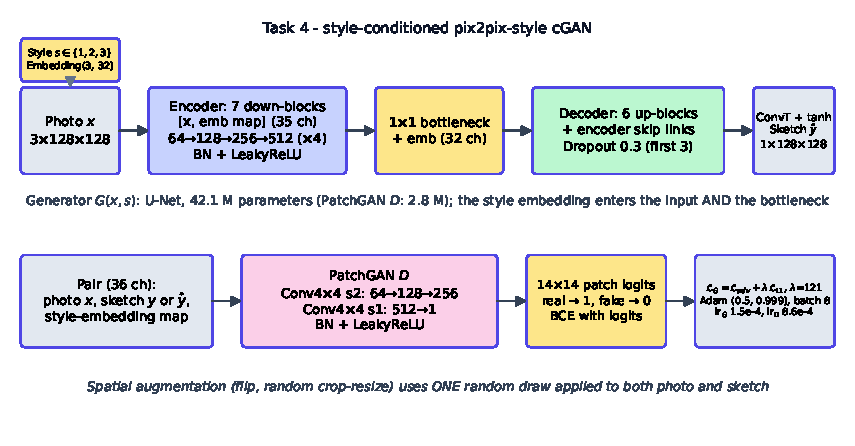
\includegraphics[width=\textwidth]{arch_task4.pdf}
\caption{Style-conditioned cGAN: U-Net generator with a style embedding in the input and the bottleneck, and PatchGAN discriminator.}\label{fig:arch4}
\end{figure*}

\subsection{Losses and training}
The discriminator is trained with binary cross-entropy on logits to label real pairs $(x,y,s)$ as one and generated pairs $(x,G(x,s),s)$ as zero; its real and fake losses are recorded separately. The generator minimises
\begin{equation}
\mathcal{L}_G=\mathcal{L}_{adv}+\lambda_{L1}\,\mathcal{L}_{L1}\bigl(y,G(x,s)\bigr),
\end{equation}
the adversarial term being the discriminator's error on generated pairs. Both networks use Adam ($\beta_1=0.5$, $\beta_2=0.999$). Optuna tuned the generator and discriminator learning rates, batch size, base channel count, dropout, style-embedding size and $\lambda_{L1}$ with 15-epoch trials on all 899 training pairs (three completed, five pruned). The selected configuration (generator learning rate $1.5\times10^{-4}$, discriminator learning rate $8.6\times10^{-4}$, batch 8, 64 base channels, dropout 0.30, embedding size 32, $\lambda_{L1}=121$) was then trained for the full 100 epochs, recording the discriminator real and fake losses, the generator adversarial and L1 losses and the validation L1, SSIM and PSNR separately for every epoch (Fig.~\ref{fig:curves4}). Every ten epochs the same eight validation photographs are rendered in all three styles and logged to MLflow (Fig.~\ref{fig:prog}), so the development of the generator can be inspected over time.

\begin{figure*}[t]
\centering
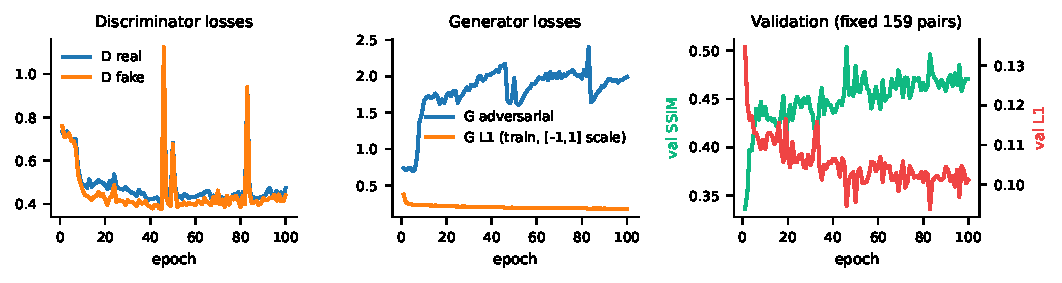
\includegraphics[width=\textwidth]{curves_task4.pdf}
\caption{Task 4 training: discriminator and generator losses, and validation SSIM and L1 (fixed validation pairs).}\label{fig:curves4}
\end{figure*}

\begin{figure*}[t]
\centering
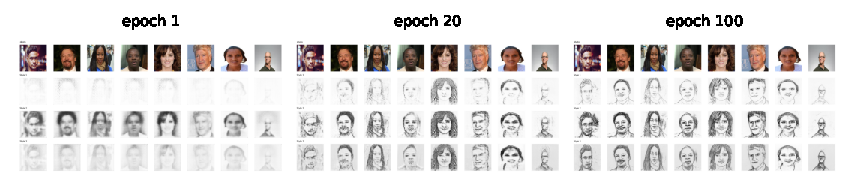
\includegraphics[width=\textwidth]{task4_progress.pdf}
\caption{The same eight validation photographs (top row of each panel) rendered by the generator in styles 1, 2 and 3 after epochs 1, 20 and 100.}\label{fig:prog}
\end{figure*}

\subsection{Results}
On the 1,046 official test pairs the selected model reaches L1 \nFourLOne{}, SSIM \nFourSSIM{} and PSNR \nFourPSNR{}\,dB (Table~\ref{tab:task4}, Fig.~\ref{fig:ex4}). The error differs strongly between styles: style~2 has an L1 error of \nFourLOnesTwo{} against \nFourLOnesOne{} for style~1 and \nFourLOnesThree{} for style~3, because its reference sketches use heavy dark strokes which a soft generator cannot match pixel by pixel, while style~1 and style~3 are lighter. The test styles are imbalanced (619, 381 and 46 pairs), so the style-3 figures rest on few samples. Each style is visibly different for the same photograph (Fig.~\ref{fig:styles}): style~2 is darkest and heaviest, style~1 lightest.

\begin{table}[t]
\centering
\caption{Task 4 on the official FS2K test set. The last row is a second training recipe (photo-only brightness/contrast jitter and learning-rate decay) that was tried and rejected because it was worse.}\label{tab:task4}
\small
\adjustbox{max width=\columnwidth}{\begin{tabular}{lrccc}
\toprule
Test subset & Pairs & L1 & SSIM & PSNR (dB) \\
\midrule
Style 1 & 619 & 0.0791 & 0.534$\pm$0.107 & 17.55 \\
Style 2 & 381 & 0.1522 & 0.395$\pm$0.082 & 12.47 \\
Style 3 & 46 & 0.0656 & 0.600$\pm$0.074 & 18.90 \\
\midrule
all (selected model) & 1046 & 0.1051 & 0.486 & 15.76 \\
all (rejected variant) & 1046 & 0.1112 & 0.451 & 15.23 \\
\bottomrule
\end{tabular}
}
\end{table}

\begin{figure*}[t]
\centering
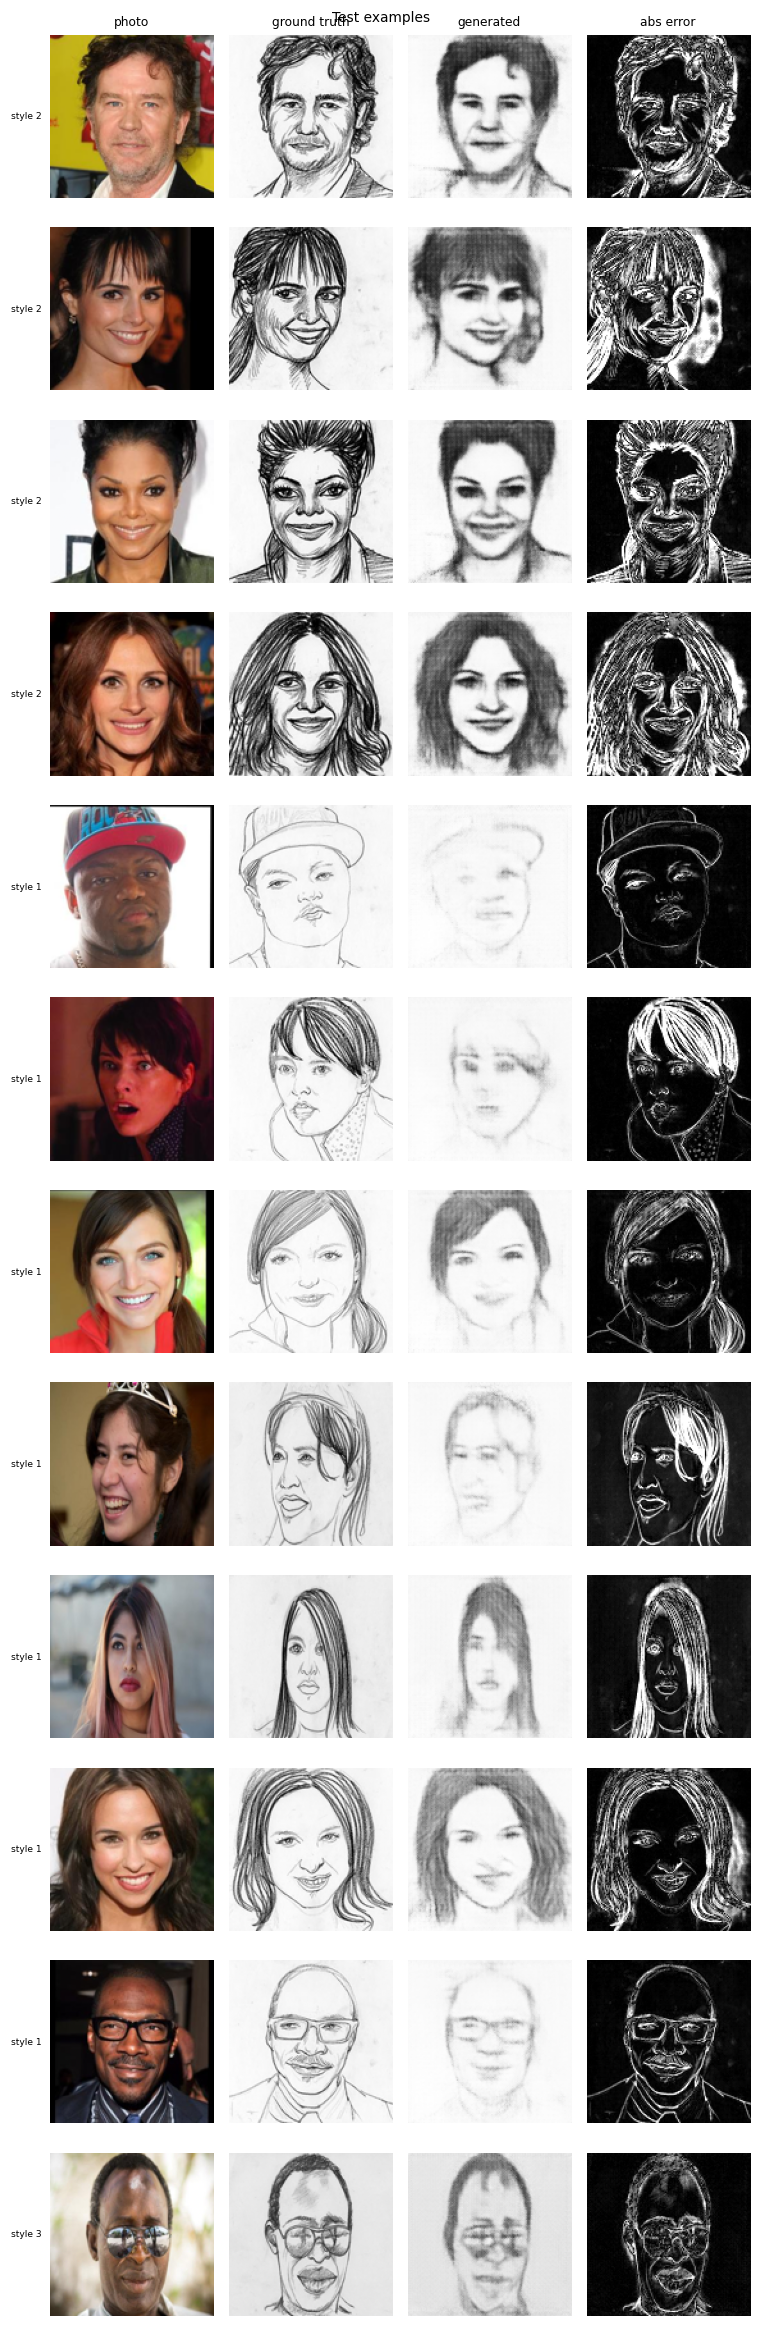
\includegraphics[width=0.78\textwidth]{task4_examples.png}
\caption{Test examples: photograph, ground-truth sketch, generated sketch and absolute error (twelve pairs spread over the test set).}\label{fig:ex4}
\end{figure*}

\begin{figure}[t]
\centering
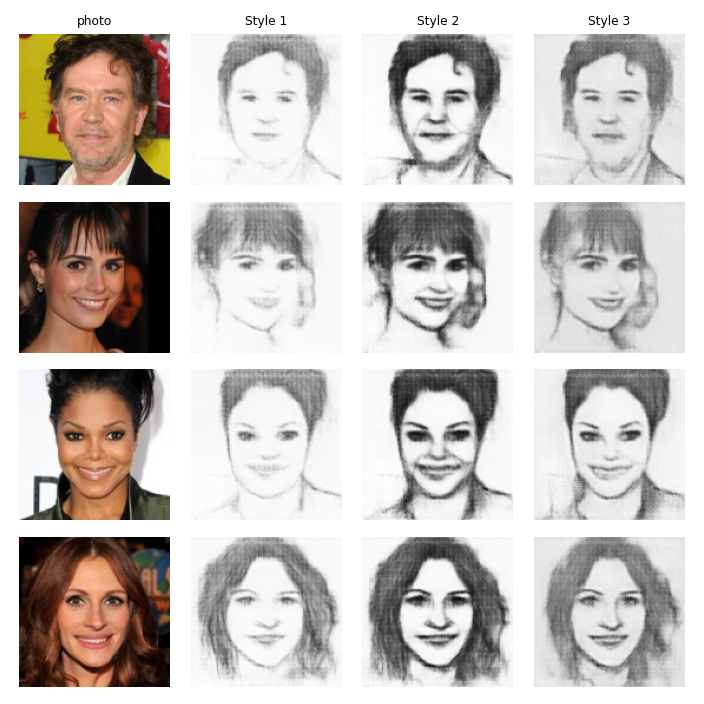
\includegraphics[width=\columnwidth]{task4_styles.png}
\caption{One photograph rendered in the three styles.}\label{fig:styles}
\end{figure}

\textbf{Why the sketches are soft.} Compared with the real sketches the generated ones are smoother (Fig.~\ref{fig:ex4}); we measured it. The average gradient magnitude of the generated sketches is only \nSharpShareAll\% of that of the real sketches (Table~\ref{tab:sharp}). A sharper input helps a little and a blurred input hurts a little (Table~\ref{tab:sens}), but the effect is small next to the 63\% gap, so the limit lies in the training rather than in the $128\times128$ input. Two causes are consistent with the evidence. With only 899 training pairs and $\lambda_{L1}=121$ the L1 term dominates and regresses towards an average stroke; and in the selected Optuna trial the discriminator stayed close to chance for the whole 15 epochs (real and fake loss near $\ln 2\approx0.69$), so the adversarial term contributed little; in the 100-epoch run it did learn to separate real from fake (losses fell to about 0.4 and the generator's adversarial loss rose to about 2, Fig.~\ref{fig:curves4}), but the generator's L1 term still dominates the objective. This is the perception--distortion trade-off~\cite{blau2018}: pixel metrics reward smooth outputs. A second recipe (photo-only brightness and contrast jitter, linear learning-rate decay) did not help (SSIM \nFourSSIMv{}, L1 \nFourLOnev{}) and was discarded. Stronger adversarial or perceptual losses, more data, or a higher resolution are the obvious next steps and were not explored.

\begin{table}[t]
\centering
\caption{Edge strength (mean gradient magnitude) of real and generated sketches on the FS2K test set.}\label{tab:sharp}
\small
\adjustbox{max width=\columnwidth}{\begin{tabular}{lrccc}
\toprule
Test subset & Pairs & Real sketch edge strength & Generated & Generated / real \\
\midrule
Style 1 & 619 & 0.0735 & 0.0267 & 36\% \\
Style 2 & 381 & 0.1506 & 0.0554 & 37\% \\
Style 3 & 46 & 0.0613 & 0.0368 & 60\% \\
\midrule
all & 1046 & 0.1011 & 0.0376 & 37\% \\
\bottomrule
\end{tabular}
}
\end{table}

\begin{table}[t]
\centering
\caption{Sensitivity of the generated edge strength to the sharpness of the input photograph.}\label{tab:sens}
\small
\adjustbox{max width=\columnwidth}{\begin{tabular}{lcc}
\toprule
Input photo (300 test faces) & Generated edge strength & L1 to real sketch \\
\midrule
input blurred (Gaussian, r=1.5) & 0.0346 & 0.1108 \\
input as is & 0.0381 & 0.1084 \\
input sharpened (unsharp mask) & 0.0436 & 0.1091 \\
\bottomrule
\end{tabular}
}
\end{table}

\begin{figure}[t]
\centering
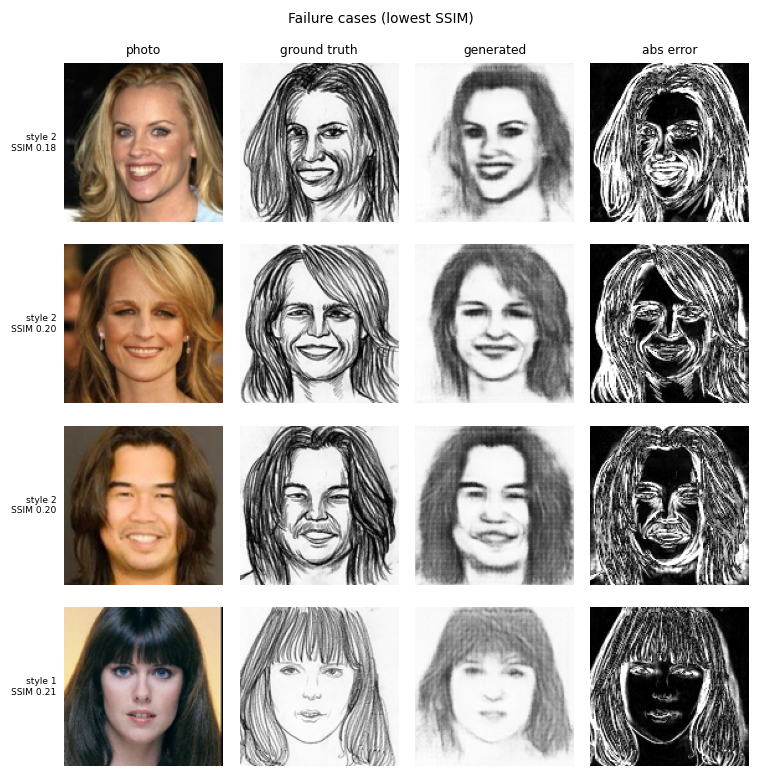
\includegraphics[width=\columnwidth]{task4_failures.png}
\caption{The four test pairs with the lowest SSIM.}\label{fig:fail4}
\end{figure}

\textbf{Failure cases.} Figure~\ref{fig:fail4} shows the four test pairs with the lowest SSIM (0.18--0.21). Three are style~2 portraits with long hair: the reference sketches draw the hair with dense, dark, hand-drawn strokes, while the generator renders it as a smooth grey mass and draws the face softly (SSIM 0.18, 0.20, 0.20). The fourth is a style~1 portrait with long hair and bangs, where the reference consists of thin, crisp lines and the generated sketch is pale and blurred (0.21). The faces remain recognisable, so these are failures of stroke detail, not of identity. The error maps light up along every reference stroke: a thin line that is missing or displaced by a few pixels costs a large pixel error, which is why pixel metrics punish a soft generator so heavily on hair-rich, style~2 subjects.

\section{Hyper-parameter Optimisation with Optuna}\label{sec:optuna}
Every task has its own Optuna study (TPE sampler, seed 42, studies stored in SQLite under \code{optuna\_studies/}, every trial also logged to MLflow). Trials are deliberately short and use sub-samples of the training data so that the search is affordable; the selected configuration is then retrained on all training data for the full schedule. Table~\ref{tab:space} lists the complete search spaces, Table~\ref{tab:optuna} the number of completed and pruned trials and the best trial of each study, Table~\ref{tab:selected} the final configurations, and Fig.~\ref{fig:optuna} the study histories. Pruning (median rule) stopped poorly performing trials early in Tasks 1, 2 (classifier), 3 and 4; the shared specialist search is not pruned because each trial trains three models and offers no single intermediate value.

\begin{table*}[t]
\centering
\caption{Complete Optuna search spaces (log = log-uniform, U = uniform, $\{\cdot\}$ = categorical). Channel options c16, c32, c48 denote the four-stage widths $(16,32,64,128)$, $(32,64,128,256)$ and $(48,96,192,384)$.}\label{tab:space}
\small
\begin{tabular}{p{2.9cm}p{9.0cm}p{4.5cm}}
\toprule
Study & Searched parameters & Trial budget and objective \\
\midrule
Task 1 (final) & lr log$[3\text{e-}4,3\text{e-}3]$; batch $\{16,32,64\}$; latent channels $\{32,64,128,256\}$; channels $\{$c16, c32, c48$\}$; dropout U$[0,0.15]$; $\alpha$ U$[0.2,0.95]$ & 12 trials $\times$ 6 epochs on 1,000 images; validation $0.5\mathcal{L}_1+0.5(1-\mathrm{SSIM})$ \\
Task 1 (first) & as above but dropout U$[0,0.3]$ and latent channels $\{16,32,64,128\}$ & 8 trials $\times$ 3 epochs on 600 images \\
Task 2 classifier & lr log$[3\text{e-}4,3\text{e-}3]$; batch $\{16,32,64\}$; channels $\{$c16, c32, c48$\}$; dropout U$[0,0.5]$; weight decay log$[10^{-6},10^{-2}]$ & 8 trials $\times$ 4 epochs on 1,000 images; validation macro-F1 (maximised) \\
Task 2 specialists & as Task 1; $\alpha$ U$[0.2,0.95]$ (first run) and U$[0.55,0.95]$ (final run) & 8 trials, each training all three specialists for 6 epochs on 1,000 images; mean validation objective \\
Task 3 & joint lr log$[10^{-5},5\text{e-}4]$; temperature $\tau$ log$[0.3,3]$; $\lambda_c$ log$[0.01,2]$; $\lambda_b$ U$[0,2]$; $\alpha$ U$[0.2,0.95]$ (first) and U$[0.55,0.95]$ (final) & 8 trials $\times$ (1 warm-up + 3 joint epochs) on 1,000 images; validation objective \\
Task 4 & $\mathrm{lr}_G$, $\mathrm{lr}_D$ log$[5\text{e-}5,10^{-3}]$; batch $\{8,16,32\}$; base channels $\{32,48,64\}$; dropout U$[0,0.5]$; embedding size $\{8,16,32\}$; $\lambda_{L1}$ log$[10,200]$ & 8 trials $\times$ 15 epochs on all 899 pairs; validation $0.5\,\mathrm{L1}+0.5(1-\mathrm{SSIM})$ \\
\bottomrule
\end{tabular}
\end{table*}

\begin{table}[t]
\centering
\caption{Optuna studies: trials, completed and pruned counts, best trial (studies marked ``first'' or ``rejected'' are kept as evidence).}\label{tab:optuna}
\small
\adjustbox{max width=\columnwidth}{\begin{tabular}{lrrrrr}
\toprule
Study & Trials & Completed & Pruned & Best trial & Best value \\
\midrule
Task 1 universal AE & 12 & 6 & 6 & \#9 & 0.2622 \\
Task 2 classifier & 8 & 4 & 4 & \#1 & 0.9243 \\
Task 2 specialists (first run) & 8 & 8 & 0 & \#6 & 0.2826 \\
Task 2 specialists (final, $\alpha\geq0.55$) & 8 & 8 & 0 & \#6 & 0.2816 \\
Task 3 soft MoE (first run) & 8 & 4 & 4 & \#0 & 0.1135 \\
Task 3 soft MoE (final, $\alpha\geq0.55$) & 8 & 4 & 4 & \#0 & 0.1108 \\
Task 4 cGAN (selected) & 8 & 3 & 5 & \#0 & 0.3139 \\
Task 4 cGAN (rejected variant) & 12 & 5 & 7 & \#0 & 0.3077 \\
\bottomrule
\end{tabular}
}
\end{table}

\begin{table}[t]
\centering
\caption{Selected configuration of each model.}\label{tab:selected}
\small
\adjustbox{max width=\columnwidth}{\begin{tabular}{lp{6.3cm}}
\toprule
Model & Selected configuration \\
\midrule
Task 1 & lr=4.61e-04, batch\_size=16, bottleneck\_dim=32, channels=c48, dropout=1.04e-03, alpha=0.583 \\
Classifier & lr=1.53e-03, batch\_size=32, channels=c16, dropout=0.152, weight\_decay=1.26e-04 \\
Specialists & lr=6.85e-04, batch\_size=32, bottleneck\_dim=32, channels=c48, dropout=0.071, alpha=0.598 \\
Soft MoE & lr=4.33e-05, temperature=2.678, w\_cls=0.483, w\_bal=1.197, alpha=0.612 \\
cGAN & lr\_g=1.54e-04, lr\_d=8.63e-04, batch\_size=8, base=64, dropout=0.301, emb\_dim=32, lambda\_l1=121.069 \\
\bottomrule
\end{tabular}
}
\end{table}

\begin{figure*}[t]
\centering
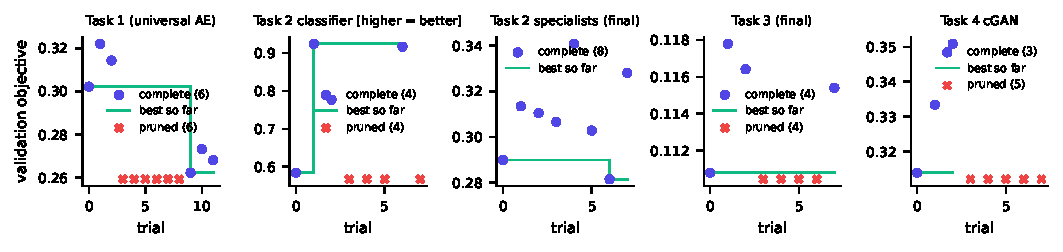
\includegraphics[width=\textwidth]{optuna_overview.pdf}
\caption{Optuna studies of the final configurations: objective value of completed trials (dots), best value so far (line) and pruned trials (crosses along the bottom).}\label{fig:optuna}
\end{figure*}

Three search-related lessons are worth recording. First, short trials favour configurations that learn fast early, which is how the first Task~1 search selected a high dropout rate that later under-fitted (Section~\ref{sec:t1}). Second, an objective made of L1 and SSIM cannot see colour loss, so the first specialist search selected an SSIM-heavy $\alpha$ that later discarded colour (Section~\ref{sec:colour}); constraining a parameter range after inspecting outputs is legitimate only when it is reported, as it is here. Third, with 8--12 trials per study the searches are compact: they find good, not optimal, settings.

\section{Application, Deployment and Tracking}\label{sec:app}
\textbf{Interface design.} The interface was designed first in Google Stitch~\cite{stitch}. A first prompt described four workspaces with a sidebar, input and corruption cards, result panels and a system-information area; Stitch returned four screens and a design system (indigo, Inter, white rounded cards). Using them, we found that the controls and Run button sat below the fold, so a run needed scrolling down to choose options and back up to see the result. A second prompt asked for a layout where everything for one run fits on one laptop screen (narrow control panel with a pinned Run button, large results on the right). Both rounds and the project page are shown in Fig.~\ref{fig:stitch}; the prompts are in \code{stitch\_design/PROMPTS.md}. The exported HTML holds invented data (GPU model, LPIPS), so only its structure, colours and typography were re-implemented as React components that show real data.

\begin{figure*}[t]
\centering
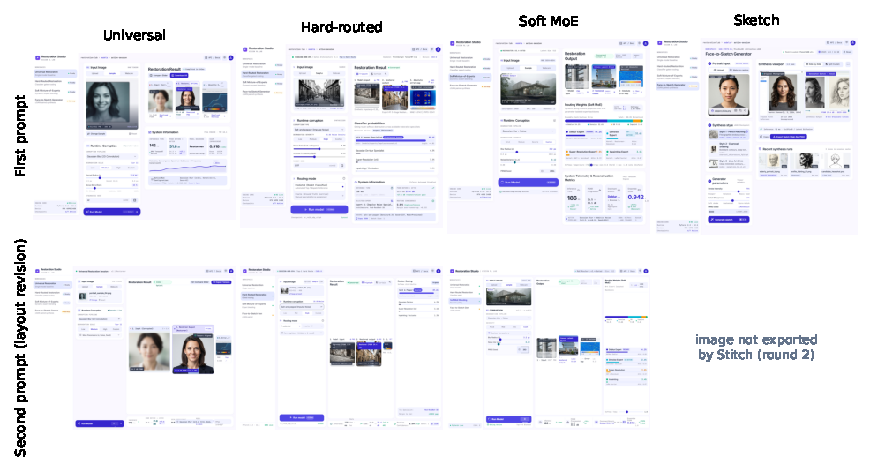
\includegraphics[width=0.49\textwidth]{stitch_montage.pdf}\hfill
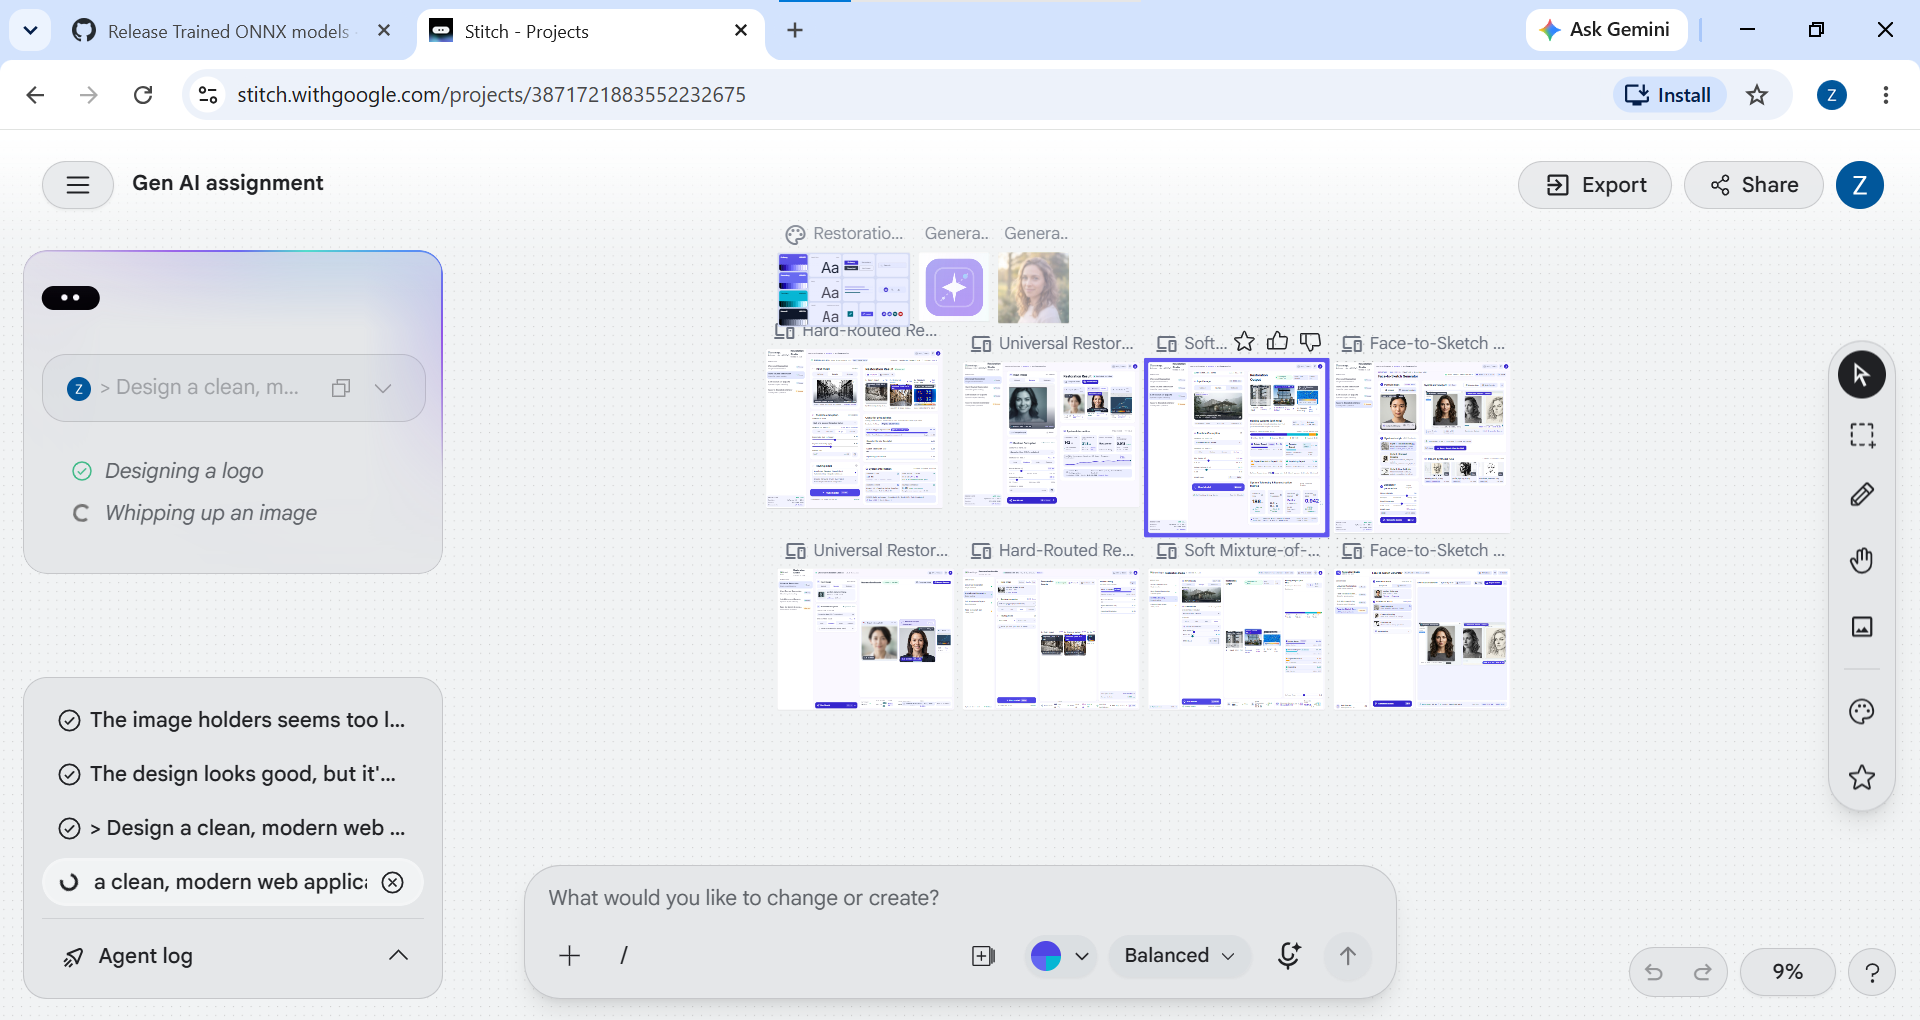
\includegraphics[width=0.49\textwidth]{stitch_project.png}
\caption{Left: Stitch designs of the first prompt (top) and the layout revision (bottom). Right: the Stitch project page with both rounds and the prompt list.}\label{fig:stitch}
\end{figure*}

\textbf{Front end and back end.} The React~18 / Vite / Tailwind front end has four workspaces (Fig.~\ref{fig:screens}): the user uploads an image, picks a built-in test sample or (for sketches) uses the webcam, chooses a corruption and severity (or custom sliders and a seed) or none, and presses Run. Results show the model input, output, absolute error map, inference time and corruption settings; hard routing adds the four classifier probabilities, the predicted corruption, the selected expert and oracle/predicted mode; the mixture adds the four weights, a stacked contribution bar and the dominant branch; sketches show photograph and sketch side by side with a download button. A browser measurement showed that at $1366\times768$ and $1920\times1080$ the Run button is always visible and the page does not scroll. The FastAPI service loads the seven ONNX models once and offers \code{/api/health}, \code{/api/restore/universal}, \code{/hard}, \code{/soft} and \code{/api/sketch}. It validates uploads (type, 10~MB and 40~megapixel limits, decodability, style and slider ranges), preprocesses exactly as in training, applies corruptions with a NumPy port of the training code, runs ONNX Runtime on the CPU and returns images, routing information and timings; a missing model gives a clear 503 message instead of a crash.

\begin{figure*}[t]
\centering
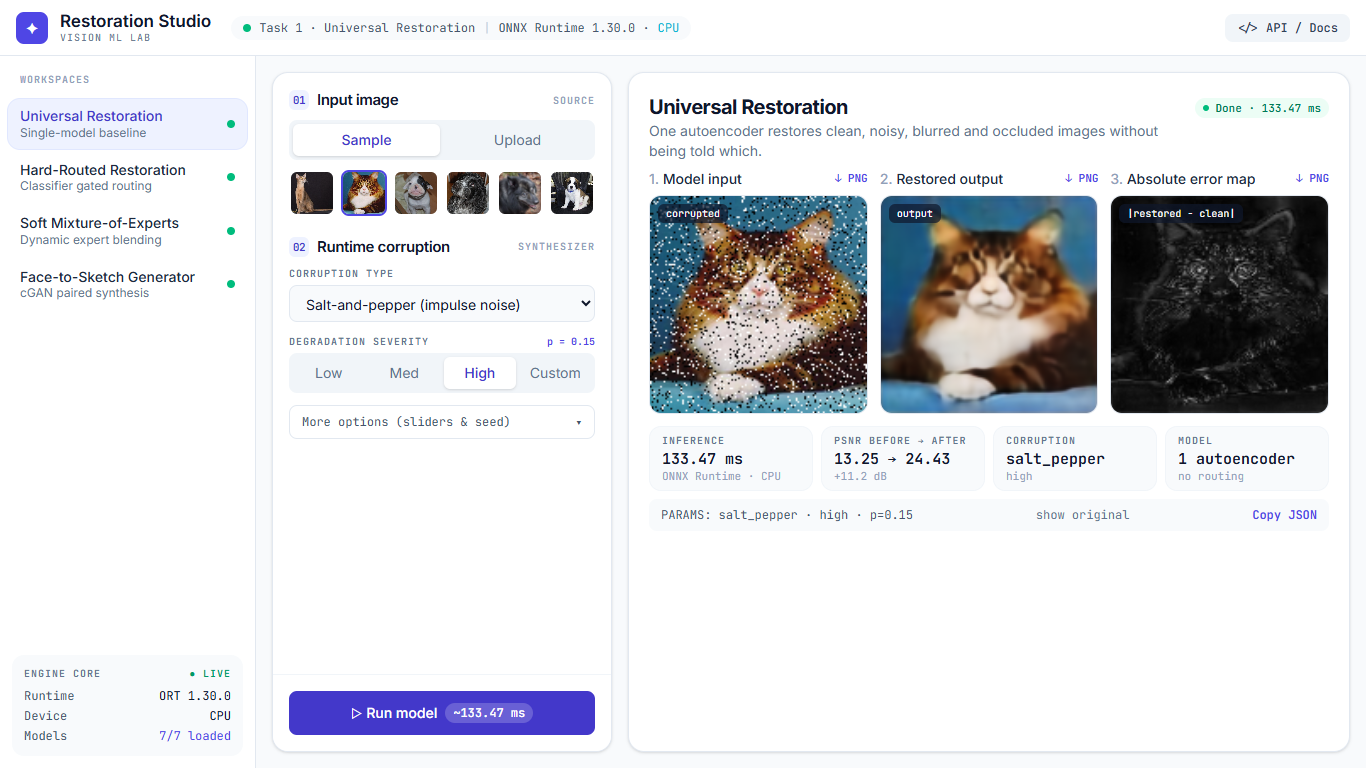
\includegraphics[width=0.36\textwidth]{app_universal.png}\hfill
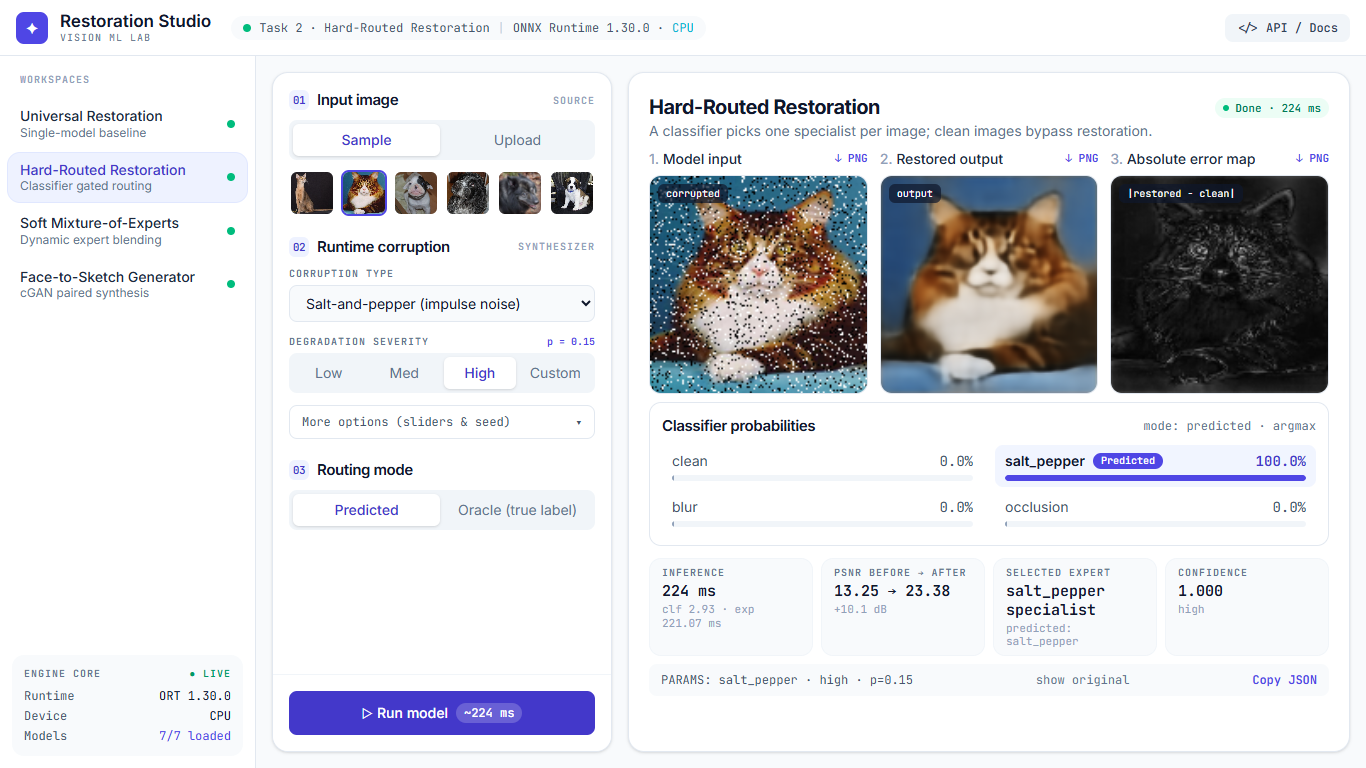
\includegraphics[width=0.36\textwidth]{app_hard.png}\\[2pt]
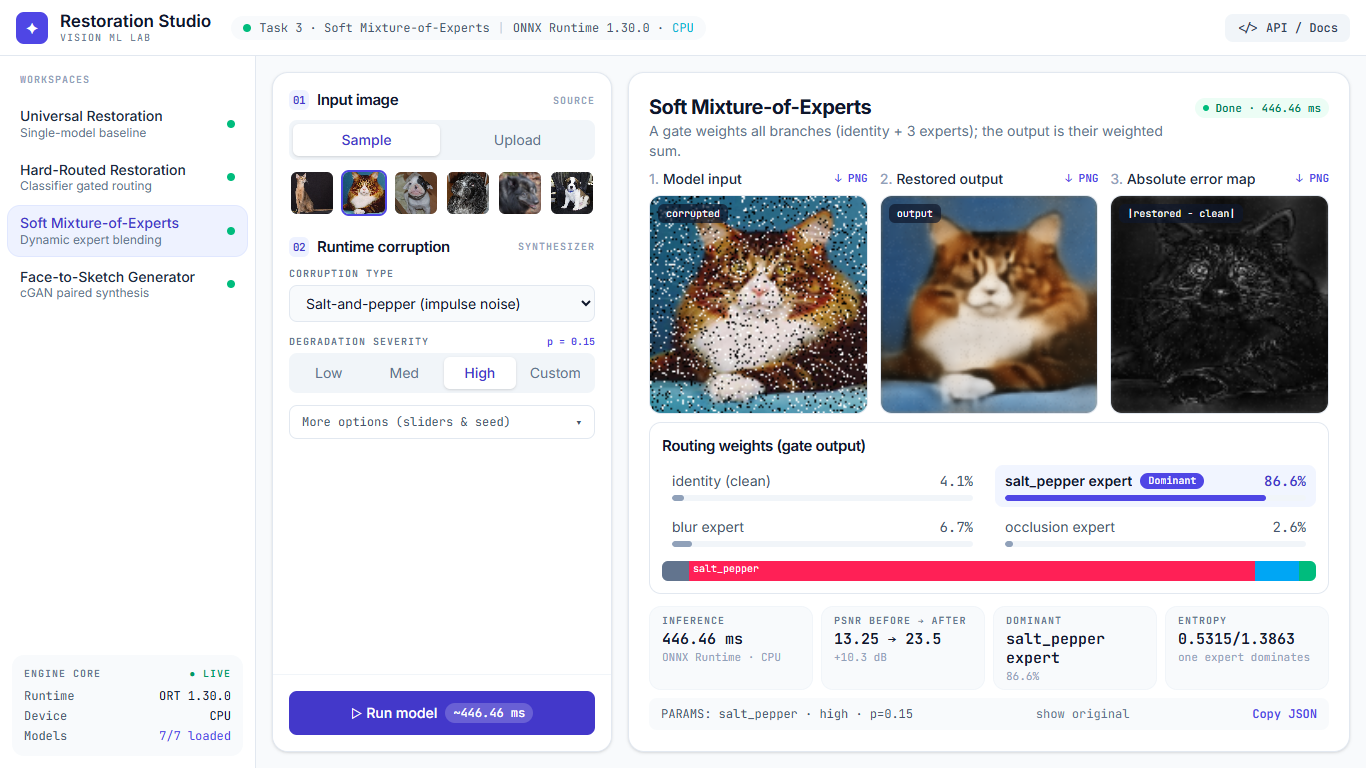
\includegraphics[width=0.36\textwidth]{app_soft.png}\hfill
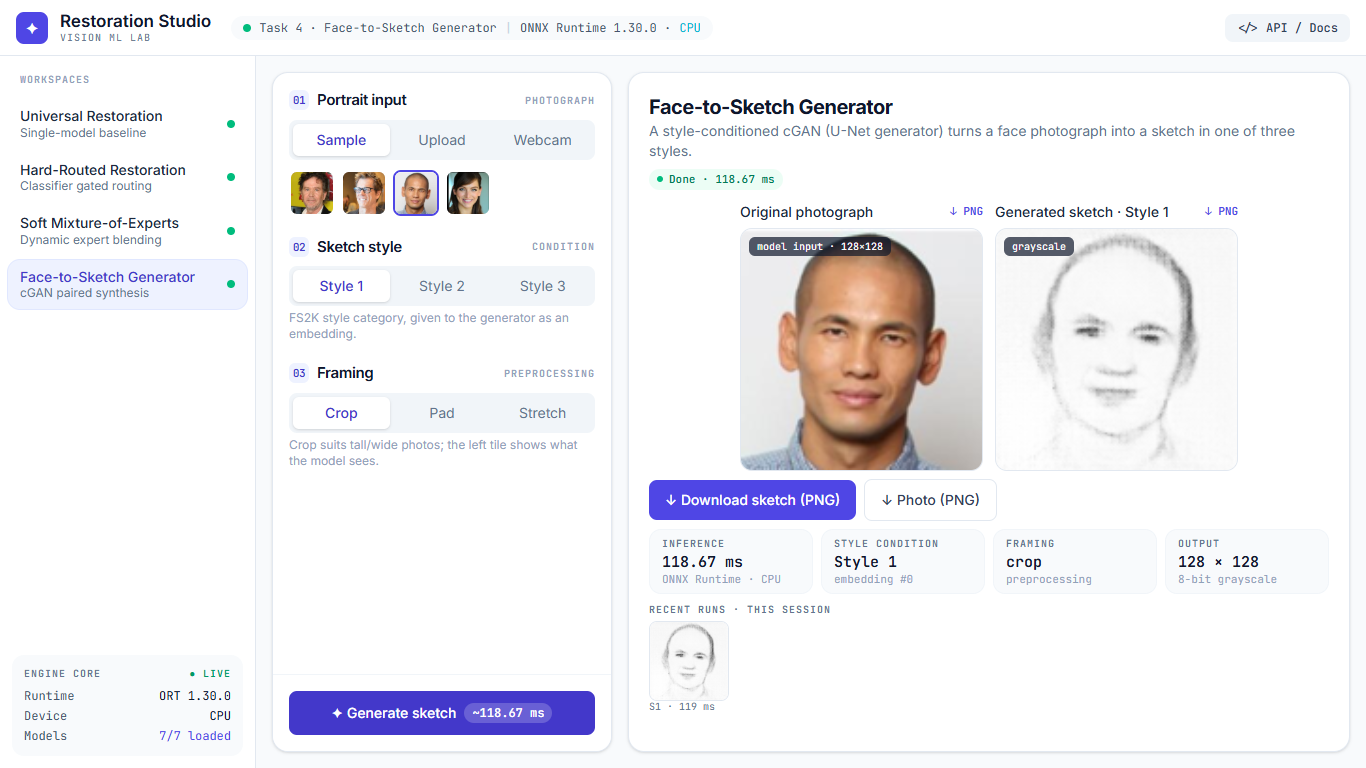
\includegraphics[width=0.36\textwidth]{app_sketch.png}
\caption{The deployed application ($1366\times768$): universal, hard-routed, soft mixture and face-to-sketch workspaces after a run on a built-in sample.}\label{fig:screens}
\end{figure*}

\textbf{ONNX.} All inference models were exported (opset 17) and compared with PyTorch on a random batch; the maximum absolute differences are all below $2.1\times10^{-6}$ (Table~\ref{tab:onnx}). The soft mixture (gate, experts, identity and mixing) is one ONNX graph returning the image and the four weights; only the cGAN generator is exported. The reported test results were also re-measured using only the deployed ONNX files, the back end's corruptions and a different SSIM implementation; SSIM agreed to four decimals on the first 300 test entries.

\begin{table}[t]
\centering
\caption{ONNX files: size, maximum absolute difference to PyTorch, CPU latency per image.}\label{tab:onnx}
\small
\adjustbox{max width=\columnwidth}{\begin{tabular}{lrrr}
\toprule
Model & Size (MB) & Max $|$PyTorch$-$ONNX$|$ & Latency (ms) \\
\midrule
Task 1 universal autoencoder & 16.1 & 5.4e-7 & 12.4 \\
Task 2 classifier & 1.2 & 2.0e-6 & 0.3 \\
Task 2 specialist (salt-and-pepper) & 16.1 & 5.7e-7 & 15.3 \\
Task 2 specialist (blur) & 16.1 & 4.5e-7 & 12.4 \\
Task 2 specialist (occlusion) & 16.1 & 5.4e-7 & 15.3 \\
Task 3 soft mixture (whole pipeline) & 49.4 & 2.4e-7 & 39.8 \\
Task 4 generator & 168.5 & 1.4e-6 & 21.1 \\
\bottomrule
\end{tabular}
}
\end{table}

\textbf{Deployment.} Two containers are built from the repository, the back end (Python, FastAPI, ONNX Runtime) and the front end (nginx serving the build and proxying \code{/api}). The model files are mounted from \code{./onnx\_models}, are not stored in Git and are fetched by \code{scripts/download\_models.py} from the \code{models-v1} release of the repository. After cloning, \code{docker compose up --build} starts the application at \code{http://localhost:3000}; an optional profile starts MLflow on port 5000. A smoke test exercises every endpoint, option and error path through the nginx address (54 checks), and the back end has 38 unit tests. \code{README.md} and \code{KAGGLE\_GUIDE.md} give the complete steps to run, retrain and evaluate.

\textbf{Experiment tracking.} Runs, Optuna trials, hyper-parameters, per-epoch losses and metrics, checkpoints and visual outputs (Task~4 sample grids every ten epochs) are recorded with MLflow in five experiments; the MLflow database and Optuna studies are in the repository (Fig.~\ref{fig:mlflow}).

\begin{figure*}[t]
\centering
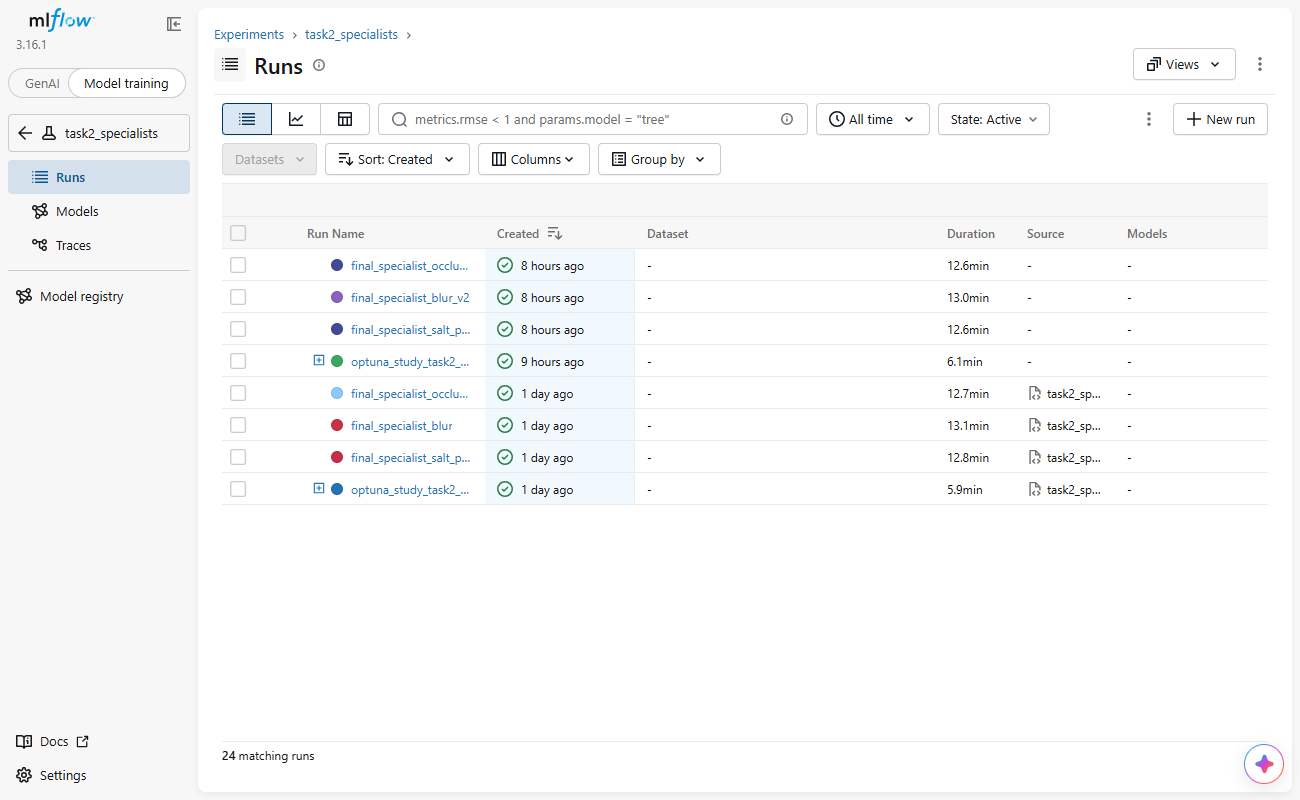
\includegraphics[width=0.36\textwidth]{mlflow_experiments.png}\hfill
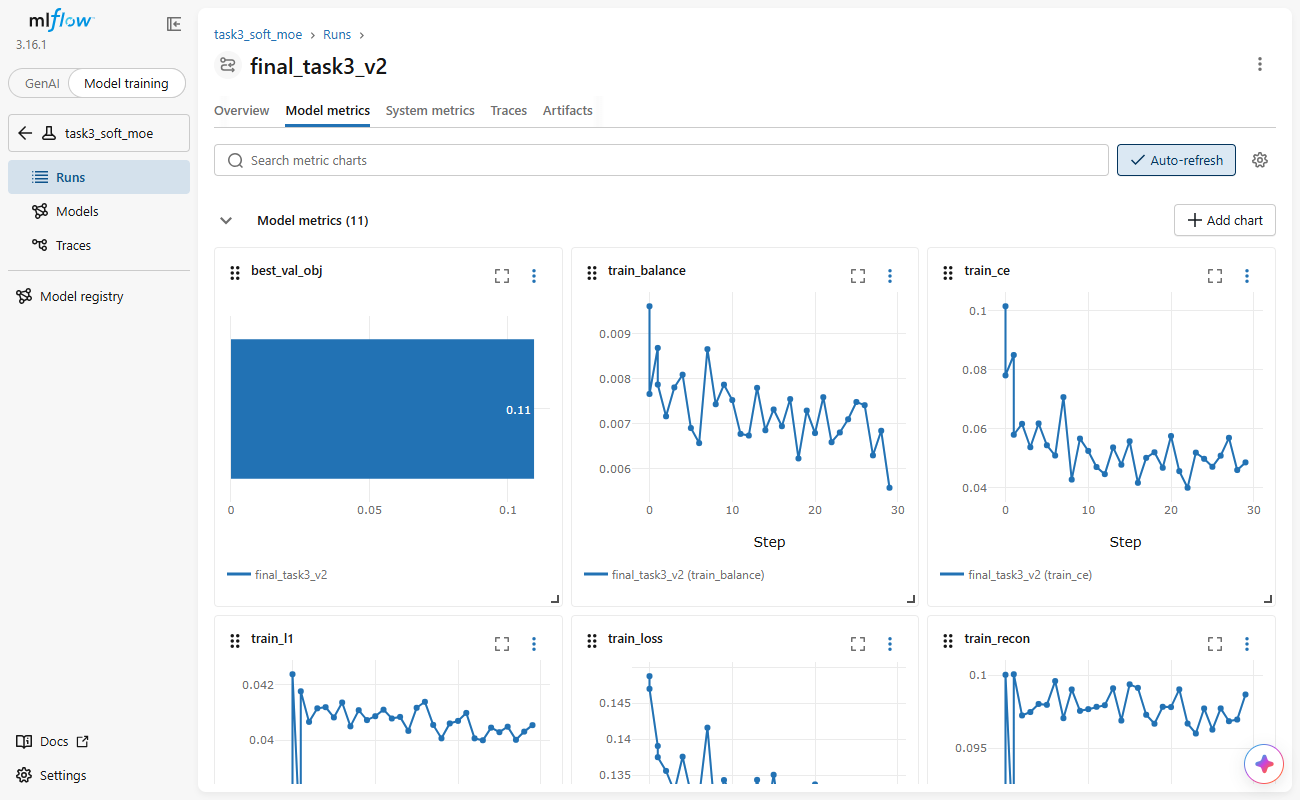
\includegraphics[width=0.36\textwidth]{mlflow_run.png}
\caption{MLflow: the experiments with their runs (left) and the metrics of one run (right).}\label{fig:mlflow}
\end{figure*}

\section{Limitations and Conclusion}\label{sec:limits}
\begin{itemize}
\item \textbf{The universal model damages inputs that need no restoration} (clean SSIM \nTOneSSIMclean{}); routing and mixing exist to avoid this, and specialisation itself did not improve corrupted cases (0.01--0.02 SSIM worse).
\item \textbf{SSIM rewards leaving small occlusions untouched,} although PSNR is about 8\,dB lower and the hole is visible, so occlusion conclusions rest on PSNR and visual inspection too. Heavy occlusion is irreversible: outputs in masked regions are plausible blur.
\item \textbf{Small searches} (8--12 trials, three completed for Task~4) find good, not optimal, settings; alternative GAN objectives were not tried. The $\alpha$ range of the final specialists and mixture was restricted after looking at the outputs.
\item \textbf{Task~3 batches} are balanced only in expectation; the classifier used exactly balanced batches.
\item \textbf{Evaluation history.} Kaggle scripts used a single-condition test manifest (3,669 inputs); the full protocol (36,690 inputs) was evaluated afterwards on the deployed ONNX models because the final training checkpoints were not archived; for the same reason the training curve of the final mixture is transcribed from the Kaggle console log. Results are from one training run per configuration, without confidence intervals.
\item \textbf{Domain.} The restoration models saw only cats and dogs and restore other subjects (such as faces) poorly; the cGAN saw frontal, near-square photographs, so photographs should be cropped.
\item \textbf{Soft sketches:} \nSharpShareAll\% of the real edge strength, and only 46 test pairs in style~3. The CPU inference was not load-tested.
\end{itemize}

\textbf{Conclusion.} A single bottleneck autoencoder restores salt-and-pepper noise well (SSIM \nInputSSIMsaltpepper{} $\to$ \nTOneSSIMsaltpepper{}) and fills occlusions plausibly (PSNR \nInPSNRocclusion{} $\to$ \nTOnePSNRocclusion{}\,dB) but damages clean and mildly blurred images. A classifier with an identity bypass removes that damage (clean SSIM \nTOneSSIMclean{} $\to$ \nHardSSIMclean{}); the jointly trained mixture does the same (\nSoftSSIMclean{}) without an inactive expert, and overall SSIM moves from \nTOneSSIMall{} to \nHardPredSSIM{} and \nSoftSSIM{}, entirely through clean inputs. Two failures found by inspecting outputs (an under-fitted first model, specialists that lost colour) and the SSIM/PSNR disagreement on occlusion show that aggregate metrics and Optuna objectives are not enough. The cGAN produces recognisable, style-dependent but soft sketches. Everything runs from one \code{docker compose up} with verified ONNX models and tracked experiments.


\appendices
\section{AI-Use Statement}\label{app:ai}
The assignment permits AI assistants provided their use is disclosed and their output is verified. This appendix identifies the tools, the tasks and how the output was tested or corrected. \todo{Author: read this appendix and change anything that does not describe exactly what you did; add the prompts you personally wrote.}

\subsection{Tools and the tasks they were used for}
\begin{itemize}
\item \textbf{Claude (web chat, Anthropic).} Produced the initial project prompt and the first code base for Tasks~1--3 (data pipeline, corruption code, models, losses, training and Optuna scripts, evaluation and ONNX export scripts).
\item \textbf{Claude Code (coding assistant, Anthropic).} Integrated and debugged that code base; wrote the Task~4 cGAN code; wrote the FastAPI back end, the React/Tailwind front end, the Docker set-up, the Kaggle instructions, the verification and screenshot scripts, the report generation scripts and a draft of this report; ran tests and measurements.
\item \textbf{Google Stitch.} Generated the interface design from two prompts (Sec.~\ref{sec:app}); its exported HTML was used as a structural reference, not as the final code.
\item \textbf{Kaggle notebooks (T4 GPU).} Compute for all training runs.
\item \textbf{Libraries.} PyTorch, Optuna, MLflow, ONNX and ONNX Runtime, scikit-learn, scikit-image, FastAPI, React, Tailwind CSS, Vite, nginx and Docker.
\end{itemize}

\subsection{How the output was tested or corrected}
\begin{itemize}
\item \textbf{Automated tests.} Corruption determinism and exact pixel counts, balanced batches, manifest reproducibility, resume-from-checkpoint equivalence (a simulated crash resumes to the same weights), equality of the back end's NumPy corruptions with the training code, 38 back-end API tests, and a 54-check end-to-end test of the running application.
\item \textbf{Numerical verification.} Every ONNX export was compared with PyTorch (differences $\le2\times10^{-6}$), and the published test results were independently re-measured from the ONNX files alone with a different SSIM implementation.
\item \textbf{Corrections made after inspecting results.} The first universal autoencoder under-fitted (SSIM \nAttemptOneSSIM{}) and was retrained with a corrected search space; the first specialists lost half the colour because Optuna chose an SSIM-heavy loss weight, which a colourfulness measurement revealed, and they were retrained with a restricted range; a second cGAN recipe was measured and rejected; stretching non-square photographs distorted sketches, so a crop option was added; the test manifest was regenerated so that each test image has all ten conditions as the assignment requires; a version-control ignore rule that silently excluded the data package was found and fixed.
\item \textbf{Claims checked against data.} Memorisation was examined by comparing training and validation scores; that final models used all training data was confirmed from the MLflow run parameters; that the test set is loaded only by the evaluation scripts was confirmed by searching the code; the layout claim (no scrolling, Run button visible) was measured in a real browser.
\item \textbf{Every number in the report} tables and in the text is generated from saved result files by scripts in \code{report/}; references were written from the cited papers' bibliographic data and should be checked against the originals.
\end{itemize}


\bibliographystyle{IEEEtran}
\bibliography{refs}

\end{document}
